\makeatletter
\newcommand{\lambdabar}{{\mathchoice
  {\smash@bar\textfont\displaystyle{0.25}{1.2}\lambda}
  {\smash@bar\textfont\textstyle{0.25}{1.2}\lambda}
  {\smash@bar\scriptfont\scriptstyle{0.25}{1.2}\lambda}
  {\smash@bar\scriptscriptfont\scriptscriptstyle{0.25}{1.2}\lambda}
}}
\newcommand{\smash@bar}[4]{%
  \smash{\rlap{\raisebox{-#3\fontdimen5#10}{$\m@th#2\mkern#4mu\mathchar'26$}}}%
}
\makeatother

\chapter{Optical Response of Gases of Stationary Atoms}

Except for the simplest examples, it is impractical to analytically solve the problem of light propagation in an atomic gas when light scattering processes need to be included. In this chapter, we will examine the principle and practice of classical simulations in several atomic configurations, and introduce some benchmark results.
 
\section{From quantum field theory to classical simulations}
\label{QFTTOCLASS}

The use of classical simulations is the main method of investigating cooperative atom responses in a dense medium within our research. Under certain conditions, such as when saturation of the atoms is negligible, this approach is both theoretically valid and practically feasible.

A field theory for light and matter under the Markov and Born approximations was introduced some time ago~\cite{PhysRevA.55.513}. Starting from the full quantum field theory, a hierarchy of equations of motion for atomic correlation functions was obtained.

Specifically, let us momentarily ignore the motion of the atoms, including possible effects of photon recoil on the atoms. Second, we take the limit of low light intensity. Third, we restrict our attention to a 
 $J_g=0\rightarrow J_e=1$ atomic transition, the simplest possible realistic optical transition scheme in three dimensions. Fourth, we assume that the incoming light is classical, i.e., a quantum field in a coherent state. We define the atomic correlation functions as
\bea
\mathbf{P}_1(;\mathbf{r}_1)&=&\langle\psi^\dagger_g(\mathbf{r}_1)\mathbf{d}_{ge}\psi_e(\mathbf{r}_1)\rangle\equiv\langle \mathbf{P}^+(\mathbf{r}_1)\rangle,\nonumber\\
\mathbf{P}_2(\mathbf{r}_1;\mathbf{r}_2)&=&\langle\psi^\dagger_g(\mathbf{r}_1)\mathbf{P}^+(\mathbf{r}_2)\psi_g(\mathbf{r}_1)\rangle,\\
\mathbf{P}_3(\mathbf{r}_1,\mathbf{r}_2;\mathbf{r}_3)&=&\langle\psi^\dagger_g(\mathbf{r}_1)\psi^\dagger_g(\mathbf{r}_2)\mathbf{P}^+(\mathbf{r}_3)\psi_g(\mathbf{r}_2)\psi_g(\mathbf{r}_1)\rangle, \nonumber\\
&&\cdots,\nonumber
\eea
and also
\bea
\rho(\br_1)\equiv\rho_1(\mathbf{r}_1)&=&\langle\psi^\dagger_g(\mathbf{r}_1)\psi_g(\mathbf{r}_1)\rangle,\nonumber\\
\rho_2(\mathbf{r}_1,\mathbf{r}_2)&=&\langle\psi^\dagger_g(\mathbf{r}_1)\psi^\dagger_g(\mathbf{r}_2)\psi_g(\mathbf{r}_2)\psi_g(\mathbf{r}_1)\rangle,\\
&&\cdots.\nonumber
\eea
Here $\psi_g$ is the quantum field operator for the lower-state (ground state) atoms. For a $J_g=0\rightarrow J_e=1$ transition it would be a boson operator, but the general scheme works just as well for fermions.  The notation $\psi_e$ stands for the three Zeeman components $m_e = -1$, 0 and 1 of the excited state, and $\mathbf{d}_{ge}$ denotes a corresponding dipole matrix element; a repeated index $e$ implies the summation over the Zeeman components.
$\mathbf{P}_k(\mathbf{r}_1,\cdots,\mathbf{r}_{k-1};\mathbf{r}_k)$ is the correlation function of the polarization at $\mathbf{r}_k$ and the atom density at $k-1$ positions $\mathbf{r}_1,\cdots,\mathbf{r}_{k-1}$, and $\rho_k$ is a $k$-point density correlation function. All of the correlation functions are normally ordered. 

From the angle of classical physics, the correlations between the atoms are induced by scattered light, which in the lowest approximation is essentially dipole radiation due to the atomic polarization. Correspondingly, for our field-theory example the response of the medium is linear and isotropic, and the equation of motion for the polarization reads
\bea
\dot{\mathbf{P}}(\mathbf{r}_1)=(i\Delta-\gamma)\mathbf{P}(\mathbf{r}_1)+i\zeta\rho(\mathbf{r}_1)\mathcal{E}_0(\mathbf{r}_1)+i\zeta\int d^3r_2\sf G(\mathbf{r}_1-\mathbf{r}_2)\mathbf{P}_2(\mathbf{r}_1;\mathbf{r}_2).
\label{CORE}
\eea
As before, $\Delta$ is the detuning from the atomic resonance, $\gamma$ is the HWHM linewidth of the transition, $\zeta=\mathcal{D}^2/\hbar$, and $\mathcal{E}_0$ is what the electric field of the driving light would be if the matter were absent. $\sf G$ is the dipole field propagator, a $3\times 3$ matrix such that $\sf G(\mathbf{r}-\mathbf{r}^\prime)\mathbf{d}$ is the usual electric field at $\mathbf{r}$ from a dipole $\mathbf{d}$ at $\mathbf{r}^\prime$.

Eq.~\eq{CORE} is the first in a hierarchy of equations. The two-atom correlation function $\mathbf{P}_2(\mathbf{r}_1;\mathbf{r}_2)$ has an analogous equation of motion that is coupled to a three-atom correlation function, which is coupled to a four-atom correlation function, and so on.

One way of making progress with the hierarchy is the decorrelation ansatz
\beq
\mathbf{P}_2(\mathbf{r}_1;\mathbf{r}_2) \simeq 
 \rho(\mathbf{r}_1){\mathbf{P}}(\mathbf{r}_2).
\eeq
This ansatz will lead to the standard electrodynamics of a polarizable medium. However, we wish to solve the entire hierarchy, and thereby include all correlations $\mathbf{P}_k(\mathbf{r}_1,\cdots,\mathbf{r}_{k-1};\mathbf{r}_k)$ that the scattering of light sets up between polarization of an atom at one position and $k-1$ ground-state atoms at other positions. To this end, the remarkable result~\cite{PhysRevA.59.649} is that the entire hierarchy may be solved by means of stochastic classical-electrodynamics simulations. We will introduce the simulation process in the following sections.

\section{Preparation}
Keeping in mind the restrictions raised in Chapter~\ref{QFTTOCLASS}, in particular a sufficiently low intensity of the driving light, we formulate our model entirely classically. At present we take all time dependent quantities to be monochromatic, and write them simply in terms of complex amplitudes. For instance, the physical electric field at the position ${\bf r}$ would be expressed in terms of an amplitude vector ${\bf E}({\bf r})$ as
\beq
{\bf E}({\bf r},t) = \half {\bf E}({\bf r}) e^{-i\omega t} + {\rm c.\,c.}
\eeq
The amplitude vectors may be complex, which allows for circularly or elliptically polarized quantities as usual. 

With the given assumptions, according to the polarizability given by Eq.~\eq{POLARIZABILITY}, the dipole moment of an atom at point $\bf r$ is
\beq
{\bf d} = -\frac{\dip^2}{\hbar(\Delta+ i\gamma)} {\bf E}({\bf r})\,,
\label{staticEtoD}
\eeq
where $\dip$ is the dipole moment matrix element. An explicit relation exists between the dipole matrix element, linewidth, and the wavenumber of resonant light $k_0 = \omega_0/c$. Now, the monochromatic light with the frequency $\omega$ need not be exactly on resonance, but dealing with near-resonant transitions in atoms we may usually ignore the difference between the wavenumber $k=\omega/c$ and the resonant wave number $k_0$. We therefore write the relation
\beq
\gamma = \frac{k^3 \dip^2}{6 \pi\hbar\epsilon_0}\,.
\eeq

The linewidth $\gamma$ describes damping of the dipole due to spontaneous emission. It has appeared more than once before, but here we have the explicit expression for the first time. Though it originates from quantum mechanics, the linewidth has a clear classical analog: An oscillating dipole radiates energy that should come from somewhere, namely, from the energy of the oscillator. Even more to the present point, the linewidth may also be viewed as a result of radiation reaction: the field of the dipole falling back on the dipole and opposing its oscillations. This kind of an argument gives a quantitatively correct damping rate for a charged harmonic oscillator, albeit in a classical analysis one needs to drop manually an infinite in-phase field driving the dipole. Quantum mechanically, the infinite field is eliminated by renormalization.

$\bf{E}(\bf{r})$ in Eq.~\eq{staticEtoD} denotes the electric field inside the sample, at the position of the atom. In traditional optics, based on the assumption of a continuous medium, this is an effective electric field with local-field corrections~\cite{jackson,optics}. However, here the atomic gas is treated as an ensemble of point-like dipolar emitters, and $\bf{E}(\bf{r})$ is simply the total field at $\bf{r}$ including the incoming light plus the dipolar fields from all other atoms~\cite{PhysRevLett.112.113603}. We will see intriguing comparisons between the two models later. 

Given the dipole moment induced on an atom, it will send out both an electric and a magnetic field that fall on the atom itself, causing radiation reaction, and on the other atoms as well. For instance, the electric field from a dipole $\bd$ at ${\bf r}_0$ is given by the familiar expression~\cite{jackson}
\bea
{\bf E}({{\bf r}; {\bf r}_0}) &=& \frac{1}{4\pi\epsilon_0}\left\{
k^2( \hat{\bf n}\times{\bf d}_{})\times \hat{\bf n}\,\frac{e^{ikR}}{R}\right.\nonumber\\
&&\left.+ [3\hat{\bf n}(\hat{\bf n}\cdot{\bf d}_{})-{\bf d}_{}]\left( \frac{1}{R^3}-\frac{ik}{R^2}\right)e^{ikR}
\right\};\\
R &=& |{\bf r}-{\bf r}_0|,\quad\hat {\bf n} = \frac{{\bf r}-{\bf r}_0}{R}\,.\label{DDIR}
\label{dipolarE}
\eea
In addition to the usual far-field radiation $\propto 1/R$ we will have to consider explicitly also the near fields $\propto 1/R^2$ and $\propto 1/R^3$.

In order to shorten the ensuing expressions, for the time being we use the same units as in the numerical calculations, setting
\beq
k = c = \hbar = \frac{1}{4\pi\epsilon_0} = 1\,.
\eeq
In particular, the unit of length derives from the free-space wavelength of the radiation $\lambda$ and equals $k^{-1}=\lambdabar=\lambda/2\pi$.
In these units the relation between the positive frequency parts of the electric and magnetic fields reads
\beq
{\bf B}({\bf r}) =-i\,\nabla\times{\bf E}({\bf r}),
\eeq
the energy density and Poynting vector at the given field position are
\bea
\hbox{\sc e} &=& \frac{1}{16\pi}\, \Re[{\bf E}\cdot{\bf E}^*+{\bf B}\cdot{\bf B}^*],\\
{\bf S} &=& \frac{1}{8\pi}\, \Re[{\bf E}\times{\bf B}^*]\,,
\eea
and  the linewidth of the transition and dipole matrix element are related by
\beq
\dip= \sqrt{\frac{3\gamma}{2}}\,.
\eeq

For a dipole $\bd$ at ${\bf r}_0$, the electric and magnetic fields of dipole radiation at position $\bf r$ are then
\beq
{\bf E}({\bf r}) = {\cal E}({\bf r},{\bf r}_0)\cdot {\bf d},\quad
{\bf B}({\bf r}) = {\cal B}({\bf r},{\bf r}_0)\cdot {\bf d},
\eeq
where $\cal E$ and $\cal B$ are $3\times3$ matrices with the elements
\bea
{\cal E}_{ij}({\bf r},{\bf r}_0) &=& \hat{\bf e}_i \cdot\left\{
(\hat{\bf n}\times \hat{\bf e}_j)\times\hat{\bf n} + [3\hat{\bf n}(\hat{\bf n}\cdot\hat{\bf e}_j)-\hat{\bf e}_j]\left( \frac{1}{R^2}-\frac{i}{R}\right)\right\}\frac{e^{iR}}{R}\,,\\
{\cal B}_{ij}({\bf r},{\bf r}) &=&\hat{\bf e}_i \cdot\hat{\bf n}\times\hat{\bf e}_j\left(1-\frac{1}{iR}\right)\,\frac{e^{iR}}{R}\,.
\eea
Here $R$ and $\hat{\bf n}$ are the distance from the source point to the field point and the unit vector pointing from the source point to the field point as before, Eq.~\eq{DDIR}, and $\hat{\bf e}_i$ are the cartesian unit vectors. On the other hand, given the electric field on an atom at ${\bf r}$ and in the new convention of units, the induced dipole moment reads
\beq
{\bf d} = \alpha\,{\bf E}({\bf r}),\quad \alpha = -\frac{3}{2(\delta+i)}\,.
\label{STEADY}
\eeq
The sole material parameter that remains is the polarizability $\alpha$ expressed in terms of the detuning in units of the natural linewidth of the transition,
\beq
\delta = \Delta/\gamma\,.
\eeq

Consider now a collection of $N$ atoms at positions ${\bf r}_n$. The electric field on an atom at ${\bf r}_n$ equals the incoming field ${\bf E}_0$ plus the dipolar field from the other atoms, which is expressed in the set of equations
\beq
{\bf E}({\bf r}_n) = {\bf E}_0({\bf r}_n)+\sum_{m\ne n} {\cal E}({\bf r}_n,{\bf r}_m)\cdot{\bf d}({\bf r}_m)\,
\eeq
or
\beq
{\bf E}({\bf r}_n) = {\bf E}_0({\bf r}_n) + \alpha \sum_{m\ne n} {\cal E}({\bf r}_n,{\bf r}_m)\cdot{\bf E}({\bf r}_m)\,.\label{FEQ}
\eeq
The latter form makes a $3N\times3N$ set of linear equations for the cartesian components of the electric field at the positions of the atoms. Given the solutions ${\{\bf E}({\bf r}_n)\}$ we then have the electric and magnetic fields everywhere in space as
\bea
{\bf E}({\bf r})&=& \bE_0({\bf r}) + \alpha \sum_{n} {\cal E}({\bf r},{\bf r}_n)\cdot{\bf E}({\bf r}_n),
\label{EF}\\
{\bf B}({\bf r}) &=& {\bf B}_0({\bf r}) + \alpha \sum_{n} {\cal B}({\bf r},{\bf r}_n)\cdot{\bf E}({\bf r}_n)\,,
\label{BF}
\eea
where ${\bf B}_0$ is the magnetic component of the incident field.

In brief, the plan of the present paper is to solve Eqs.~\eq{FEQ}, be it analytically or numerically, and study the resulting electromagnetic field, Eqs.~\eq{EF} and~\eq{BF}.

One more issue needs to be addressed: What to do with gases in which the positions of the atoms are random? Reference~\cite{PhysRevA.59.649} gives an unequivocal answer: One should generate random atomic samples in which the position correlation functions are as specified by the given $\rho_k(\br_1,\ldots,\br_k)$, in principle all the way to the order $k=N$ equal to the number of atoms, and average the results over these samples. In our practical simulations we take the atoms in a gas to be distributed randomly and independently of one another in a volume defined by the geometry of the sample. This corresponds to the factorization of the correlation functions
\beq
\rho_k(\br_1,\ldots,\br_k) = \rho(\br_1)\ldots\rho(\br_k),
\eeq
and is, in fact, a microscopic model for a Bose-Einstein condensate. Various reasons exist why the positions of the atoms could have short-range correlations, such as atom-atom interactions and boson bunching. However the associated length scales, such as scattering length and thermal de Broglie wavelength are ordinarily much smaller than the interatomic spacings that we consider, so we deem our uncorrelated model to be an excellent approximation.

\section{Example: Radiation from a single atom}
We begin with a single atom at the origin of the coordinates, ${\bf r}_1 = 0$. It is driven by an incoming plane wave that propagates in the $x$ direction and is polarized in the $z$ direction, so that we have
\beq
{\bf E}_0({\bf r}) = E_0\, \hat{\bf e}_z\,  e^{i x}\,.
\eeq
Since there are no other dipoles, the field driving the atom equals the external field
\beq
{\bf E}({\bf r}_1) = E_0\, \hat{\bf e}_z\,,
\eeq
and the dipolar fields are as usual. Writing the vector from the origin to the point of observation in terms of the spherical polar coordinates,
\bea
\hat{\bf r} &=& \sin\theta\cos\varphi\, \hat{\bf e}_x+ \sin\theta\sin\varphi\, \hat{\bf e}_y + \cos\theta\, \hat{\bf e}_z,\\
{\bf r} &=& r\,\hat{\bf r}\,,
\eea
the angular distribution of the outward flux of radiated energy at $r\gg1$ and the total radiated power are
\bea
F_1(\theta,\varphi) &=& r^2 \,\hat{\bf r}\cdot{\bf S} = \frac{9 |E_0|^2 \sin^2\theta}{32\pi(\delta^2+1)},\label{1DIPF}\\
P_1 &=& \int d\theta \sin\theta\,d\varphi\, F(\theta,\varphi) = \frac{3|E_0|^2}{4(\delta^2+1)}\label{1DIPP}\,.
\eea
These are utterly familiar results, even if they might look unusual at first sight  because of our units.

Even though this is the case of a single atom and therefore presents no enhanced radiation due to interference or cooperative effects, it is still instructive to see how the energetics works out; see also Ref.~\cite{CRA82}. Thus, the total electric and magnetic fields at the point $\br$ are written
\beq
\bE_T(\br) = \bE_D(\br) + \bE_0(\br),\, {\bf B}_T(\br) = {\bf B}_D(\br) + {\bf B}_0(\br),
\eeq
where the index $D$ denotes for the dipole radiation from the atom and index $0$ for the incoming field. The total Poynting vector therefore is
\beq
{\bf S}_T = \frac{1}{8\pi}\, \{\Re({{\bf E}_0}\times{{\bf B}_0}^*)+ \Re({{\bf E}_D}\times{{\bf B}_D}^*) + [\Re({{\bf E}_0}\times{{\bf B}_D}^*) +  \Re({{\bf E}_D}\times{{\bf B}_0}^*)]\}\,.
\eeq
The first term is due to the incoming field. When the corresponding energy flux is integrated over a surface not containing any part of the source of the incoming field, the result is obviously zero. The second term is due to the radiation of the dipole alone, as if the incoming field were not present, and provides Eqs.~\eq{1DIPF}, \eq{1DIPP} for the flux and the total radiated power. The final two terms in square brackets produce the portion of the Poynting vector that corresponds to the interference between the incoming and the dipolar fields.

At large distances the interference terms are the dominant contribution to the Poynting vector. As they are quite complicated already for such a simple case, we do not write them down, but at a fixed large distance they may vary rapidly with the angles and have a negative radial component, as if power were streaming toward the radiating dipole. One cannot guarantee that the Poynting vector is the local energy current density, as the continuity equation for energy only says that the integral of the normal component of the Poynting vector over a closed surface equals the rate of change of the energy inside that surface. Nevertheless, one can  show analytically that the total power associated with the interference term equals $-P_1$. The total power coming  out of a closed (spherical, in our explicit calculations) surface surrounding the dipole therefore equals $P_1-P_1=0$. This is as it should be, as evidently the dipole does not store or emit net energy but simply reradiates it.

\section{Example: Radiation from two atoms}
For two atoms an explicit solution for the radiation field exists no matter what are the incoming fields and the positions of the dipoles, but the general expression is complicated enough to be useless. We discuss here as an example the special case in which a plane wave polarized in the $z$ direction and propagating in the $x$ direction strikes two atoms sitting on the $z$ axis. Specifically, we have the incoming field and the two positions for the dipoles
\beq
E_0({\bf r}) = E_0\, \hat{\bf e}_z\,  e^{i x},\quad {\bf r}_{\pm} = \pm\half\,\ell\,\hat{\bf e}_z\,.
\eeq

In this case the fields at the positions of the dipoles are
\beq
{\bf E}({\bf r}_\pm) = \frac{\ell ^3}{\ell ^3+2 i \alpha  \ell e^{i \ell }-2 \alpha  e^{i \ell }}\,E_0\,\hat{\bf e}_z\,.
\label{FOD}
\eeq
Since the dipolar field diverges with decreasing distance from the dipole, one might expect that the field of one induced dipole on the other would also diverge when the dipoles approach one another, but in a sense the exact opposite holds true: For a fixed detuning and hence fixed polarizability $\alpha$, the fields are actually proportional to $\ell^3$ as $\ell\rightarrow0$.

However, fixed detuning may not be the most useful way of viewing the result. Instead, we insert the explicit expression of the polarization and write
\bea
{\bf E}({\bf r}_\pm) &=& \left\{
1 + \frac{3 e^{i\ell}(1-i\ell)/\ell^3}{\Delta(\ell)-i\gamma(\ell)}
\right\}E_0\,\hat{\bf e}_z;\\
\Delta(\ell) &=& \Delta -3  \left[\frac{\cos (\ell )}{\ell ^3}+\frac{\sin (\ell )}{\ell
   ^2}\right] \gamma,\nonumber\\
\gamma(\ell) &=&\left[1+\frac{3 \sin (\ell )}{\ell ^3}-\frac{3 \cos (\ell )}{\ell ^2}\right]\gamma \,.
\label{GAMMAL}
\eea
This shows our first instance of collective shift and broadening of the resonance of the atoms as a result of the radiation from one dipole falling on the other. The sines and cosines clearly originate from retardation, propagation delay of light between the atoms. In the limit $\ell\rightarrow0$ we have the expansions, keeping the leading terms in real and imaginary parts,
\beq
\Delta(\ell)-\Delta \simeq -\frac{3\gamma}{\ell^3},\,\gamma(\ell) \simeq 2\gamma\,.
\eeq
The shift $\Delta(\ell)-\Delta$ diverges as  $\ell^{-3}$, which clearly reflects the dipole-dipole interactions between the atoms. On the other hand, the linewidth doubles.

Moving on to the energy flux in the far field and to the radiated power, we find after some tedious algebra (even with Mathematica) the expressions
\bea
F_2 &=& \frac{9 \gamma ^2 |E_0|^2 \cos ^2\!\left[\frac{1}{2} \ell  \cos
   (\theta )\right] \sin ^2(\theta )}{8 \pi  \left[\Delta (\ell )^2+\gamma (\ell )^2\right]},\\
P_2 &=&\frac{3 \gamma\,\gamma(\ell)|E_0|^2 }{2[\Delta^2(\ell)+\gamma^2(\ell)]}\,.
\eea
The angular distribution of the radiation, normalized in such a way that $\int_0^\pi d\theta\,\sin\theta P(\theta)=1$, reads
\beq
P(\theta;\ell) = \frac{3\gamma}{2\gamma(\ell)}\cos^2\left[\frac{1}{2} \ell  \cos
   (\theta )\right] \sin ^2(\theta )\,.
\eeq
This shows the dipole radiation pattern modulated by the interference of the radiation from the two dipoles; see the demonstration in Fig.~\ref{TWOATOMS}. For $\ell=0$ we have the usual dipole radiation pattern. With increasing $\ell$ the interference first concentrates the radiation more to the $\theta=\pi$ plane perpendicular to the dipole. With increasing $\ell$ the side lobes grow numerous, and the overall angular distribution pattern rounds out.

\begin{figure}[h!]
\begin{center}
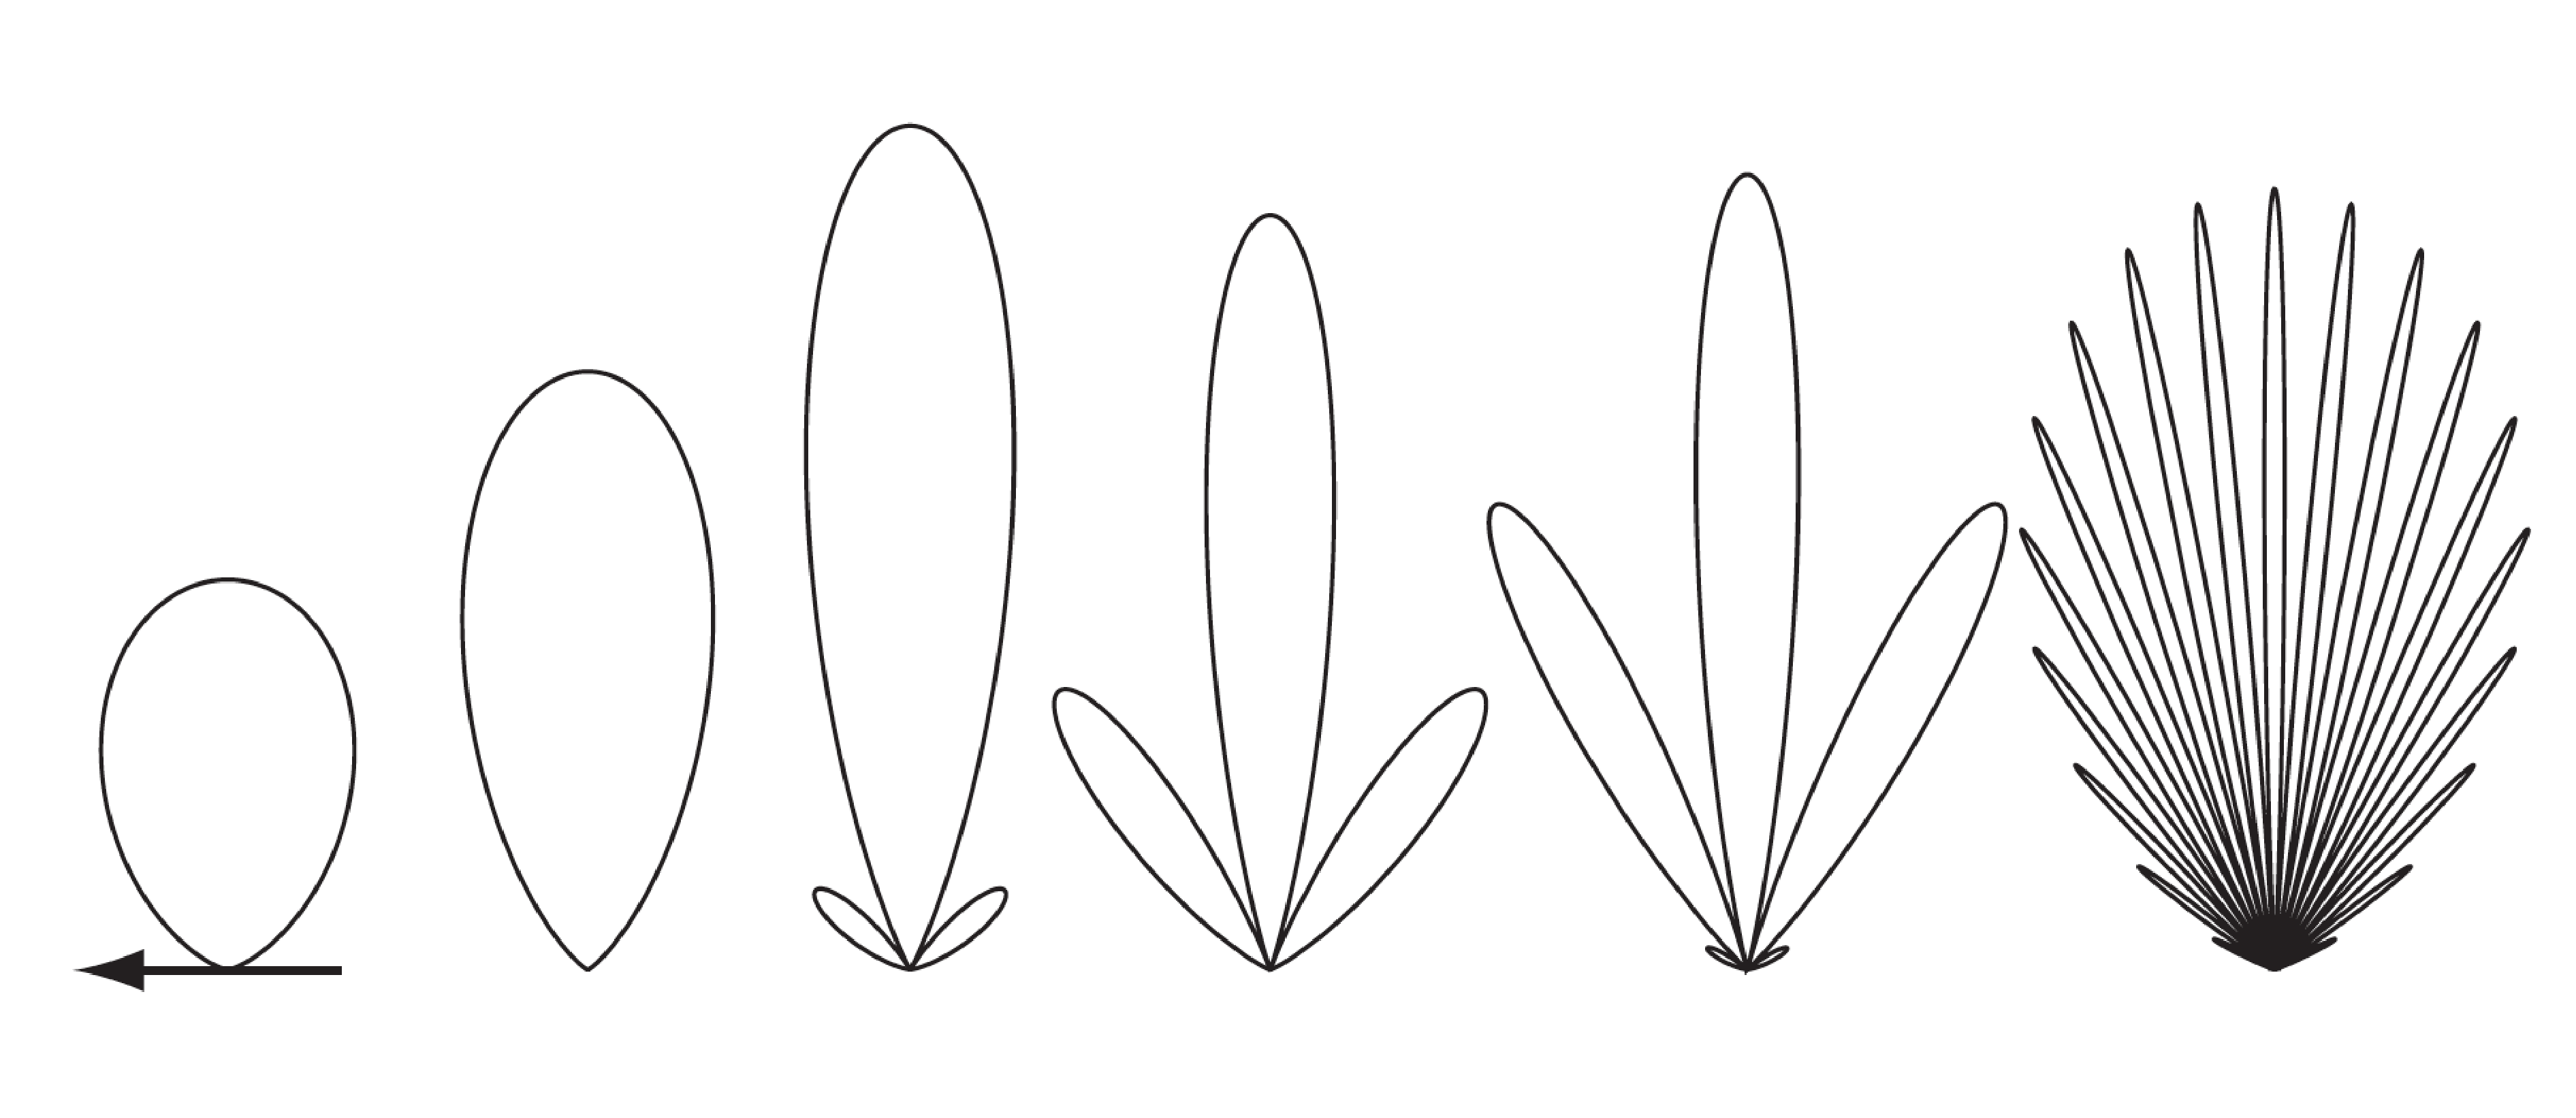
\includegraphics[width=0.8\textwidth]{two_atoms.pdf}
\end{center}
\caption[Radiation patterns for two dipoles]{Normalized radiation patterns $P(\theta;\ell)\sin\theta$ for the two dipoles for the distances between the dipoles $\ell=0,\,\pi,\,2\pi,3\,\pi,4\,\pi$, and $20\pi$ (left to right). These are a polar plots for $\theta\in[0,\pi]$,with the direction of the dipole and the $z$ axis denoted by the arrow in the $\ell=0$ graph.}
\label{TWOATOMS}
\end{figure}

As to the radiated power, the detuning from the resonance shifted by the cooperative-operative effects is the true gauge of resonance effects. We momentarily assume that this shift of reference point is implicit in the expression of the power in the two-atom radiation $P_2$, and simply replace $\Delta(\ell)\rightarrow\Delta$. On the other hand, if there were no cooperative-operative effects or interference between the radiations from the two dipoles, the total radiated power would simply be twice the radiated power from one dipole under the same driving field. The ratio of the actual two-atom power and the power from two independent dipoles
\beq
C = \frac{P_2}{2 P_1} = \frac{\gamma(\ell)[\Delta^2+\gamma^2]}{\gamma[\Delta^2+\gamma^2(\ell)]}
\eeq
is a reasonable measure of cooperativity, with $C=1$ applying to completely independent radiators.

The explicit expression follows immediately from Eq.~\eq{GAMMAL}. Because in the limit $\ell\rightarrow\infty$ we have $\gamma(\ell)\rightarrow\gamma$, we find $C\rightarrow1$ as expected. In the opposite limit $\ell\rightarrow0$ we have $\gamma(\ell)\rightarrow 2\gamma$, and the cooperative-operation of the dipoles depends in an essential manner on the detuning. If $|\Delta|\ll\gamma$, we have $C\simeq\half$. This means that on resonance the two atoms together radiate the same power as one single atom. On the other hand, with $|\Delta|\gg\gamma$, we have $C\simeq2$, and the two-atom sample radiates twice as much power as two independent atoms would. In fact, in this limit the radiated power can be expressed at all detunings as
\beq
P_2 = \frac{3 |E_0|^2}{2\{[\Delta/2\gamma]^2+1\}}\,,
\eeq
as if we had a single dipole with the dipole moment matrix element equal to $\sqrt2$ times the original dipole moment matrix element.

 Now, it is well known that on resonance the cross section for light scattering is independent of the dipole moment matrix element, so the cross section and scattered power are both independent of the dipole matrix element. On the other hand, far-off resonance the scattered power is in fact proportional to the square of the dipole matrix element times the linewidth, and as such is proportional to the fourth power of the matrix element. Hence, the power from two atoms should be four times the power from one atom, or twice the power from two independent atoms. The $\ell\rightarrow0$ limit is fully compatible with the observation that the two atoms have merged into one and the dipole matrix element has been multiplied by $\sqrt2$, with the proviso   that, as a result of atom-atom interactions, a shift of the resonance occurs that diverges in the limit $\ell\rightarrow0$.

There is an interesting little puzzle here: One would imagine that when one simply joins the two atoms, the dipole moment matrix element should be twice the matrix element for a single atom, not the multiple $\sqrt 2$. Granted, in quantum mechanics, when restricted to the state space of collective states that are invariant under the exchange of the two atoms, the factor in fact is $\sqrt2$. But here we have a completely {\em classical\/} situation. What gives?

To find the solution, let us momentarily take a variation of the classical Lorentz model for a dipole, namely two classical charged particles with charge $q$ and mass $m$ moving in the $z$ direction. Both particles are bound to their equilibrium positions with assumedly immovable neutralizing charges, so that there are restoring forces proportional to the square of the of natural frequency $\omega_0$ common to both of the oscillators. By a suitable choice of the origins of the coordinates, we make the equilibrium positions equal to zero. Nonetheless, we assume that in actuality the dipoles sit back to back as in the example of the present section, and much closer than the wavelength of the driving light from one another. The fields from one dipole, the moving charge and the stationary "nucleus", then add up to a force that attempts to move the other charge in the same $z$ direction. We characterize this force by the frequency $\Omega$. Finally, we assume that both of the dipoles are driven by the same external field $E$ at the frequency $\omega$. The equations of motion for the positive-frequency components of the positions of the two charges are then
\bea
\ddot{z}_1 = -\omega_0^2 z_1+ \Omega^2 z_2 + \frac{qE}{2m}e^{-i\omega t},\label{INDIVDIP1}\\
\ddot{z}_2 = -\omega_0^2 z_2+ \Omega^2 z_1 + \frac{qE}{2m}e^{-i\omega t}\,.
\eea
In terms of the normal modes
\beq
\eta_\pm = \frac{1}{\sqrt 2} (z_1 \pm z_2)
\eeq
the equations of motion read
\bea
\ddot{\eta}_+ &=& -(\omega_0^2-\Omega^2)\eta_+ +\frac{qE}{\sqrt2\, m} e^{-i\omega t},\label{COLLDIPP}\\
\ddot{\eta}_- &= &-(\omega_0^2+\Omega^2)\eta_-\,.
\eea
The resonance of the two modes $\eta_\pm$ are shifted in the opposite directions by the interaction between the dipoles. Besides, the ``nonradiating'' mode $\eta_-$ does not couple to the driving field at all. 

Let us now assume that there is some damping in the system that eventually leads to equilibrium, but which is otherwise negligible. For instance, assume that we drive the dipoles far-off resonance. Then no excitation of the mode $\eta_-$ is present. Moreover, a comparison of Eqs.~\eq{COLLDIPP} and~\eq{INDIVDIP1}  shows that for the same driving field strength $E$ and for the same detuning of the frequency $\omega$ from the respective resonance frequencies $\sqrt{\omega_0^2-\Omega^2}$ and  $\omega_0$, the steady-state oscillation amplitude of the collective mode $\eta_+$ would be a factor of $\sqrt 2$ larger that the amplitude of a single dipole.

This is ostensibly the $\sqrt 2$ for the collective response in quantum mechanics, but the normal modes are an auxiliary construct and as such have no a priori meaning in classical mechanics. We therefore consider the original displacement $z_1$ and $z_2$. These, in fact, oscillate in phase, and with the same amplitude as would one dipole for the same detuning from resonance. The total radiated electric field from the two dipoles will thus be twice the field from one dipole, and the radiated power is multiplied by four. Everything is as expected. The reason for the factor-of-two enhancement in radiated power is simply constructive interference of the two radiators. At least in the far-detuned case the quantum mechanical enhancement of the dipole moment matrix element by $\sqrt2$ is an illusion.


\section{Radiation power from Gaussian clouds of atoms}


\subsection{Continuous medium}

For the more general problem of $N$-atom gases, let us start with a hypothetical model with a continuous spatial distribution of atoms.

In terms of macroscopic electromagnetism, there is a monochromatic polarization of the sample
\beq
{\bf P}({\bf r},t) = \half\rho({\bf r}) \,{\bf d}({\bf r})e^{-i\omega t} + {\rm c.c.}\,,
\eeq 
where $\rho({\bf r})$ is the density of the sample  and $\bf d({\bf r})$ is the electric dipole of an atom at the position $\bf r$. Taking the atoms  to reside around the origin of the coordinates, in the far field with the distance $r\gg1$ and with $r$ much larger than the size of the sample, the terms  $\propto 1/R^2$ and $\propto 1/R^3$ in Eq.~\eq{dipolarE} are negligible and the  field  radiated by this polarization is
\bea
{\bf E}_R({\bf r})&\simeq&\frac{e^{ir}}{r} \int d^3r'\,e^{-i  \hat{\bf r}\cdot {\bf r}'}\rho({\bf r}')
\, [\hat{\bf r}\times{\bf d}({\bf r}')]\times\hat{\bf r}\,;
\label{SCATFIELD}
\eea
$\hat{\bf r}={\bf r}/r$ is the unit vector that points from the source at $\simeq 0$ to the field point. 

For easy analysis, we model the density with a Gaussian,
\beq
\rho({\bf r}) = \frac{3\sqrt3N}{2\sqrt2\pi^{3/2} R^3}\, e^{-\frac{3r^2}{2R^2}}\,,
\label{CONT_DEN}
\eeq
where $N$ is the atom number and $R$ is the size scale of the sample. The parametrization is chosen in such a way that the rms value of $|\br|$ equals $R$. In the limit $R\gg1$ there will be a narrow cone of radiation around the direction of the incoming beam; let us denote the angle from the incident beam by $\theta$.  

For a tangible example, let us take a $\sigma_+$ circularly polarized plane wave propagating in the $z$ direction, writing
\beq
\bE_0(\br) = E_0\, e^{iz}\,\hat{\bf e}_+;\quad \hat{\bf e}_+=-\frac{1}{\sqrt{2}}(\hat{\bf e}_x + i \hat{\bf e}_y)\,.
\label{incomingE}
\eeq
The key assumption here is that the incoming light dominates even inside the sample. Accordingly, we write the dipole moment of an atom at $\br$ simply as
\bea
{\bf d}({\bf r})=\alpha\bE_0(\br)=\alpha E_0\, e^{iz}\,\hat{\bf e}_+.
\eea

Now we turn back to the radiated field:
\bea
{\bf E}_R({\bf r})&=&\frac{e^{ir}}{r}\int d^3r^{\prime} e^{-i\hat {{\bf n}} \cdot {\bf r}^{\prime}} \rho({\bf r^\prime}) [ \hat { \bf n} \times  {\bf d}({\bf r}^{\prime}) ]  \times \hat {\bf n}\nonumber\\
&=&\frac{3\sqrt{3}\alpha NE_0e^{ir}[ (\hat { \bf n} \times \hat{{\bf e}}_+)  \times \hat {\bf n}]}{2\sqrt{2}\pi ^{3/2}R^3r}\int d^3r^{\prime} e^{-i\hat {{\bf n}} \cdot {\bf r}^{\prime}}e^{iz}e^{\frac{-3r^{\prime2}}{2R^2}}\nonumber\\
&=&\frac{\alpha NE_0e^{ir-\frac{1}{3}R^2(1-\cos \theta)}}{r}[ (\hat { \bf n} \times \hat{{\bf e}}_+)  \times \hat {\bf n}].
\eea
The magnitude of the Poynting vector is 
\bea
S_R({\bf r})&=&\frac{|{\bf E}_R|^2}{8\pi}=\frac{\left|\alpha\right|^2N^2 E_0^2 e^{-\frac{2}{3}R^2(1-\cos \theta)}|(\hat { \bf n} \times \hat{\bf e}_+) \times \hat {\bf n} |^2}{8 \pi r^2} \nonumber\\
&=&\frac{\left|\alpha\right|^2N^2 E_0^2 e^{-\frac{2}{3}R^2(1-\cos \theta)} (1+\cos^2 \theta)}{16 \pi r^2}.  
\eea
The total power of the radiation is readily obtained as
\bea
P_R&=&\int r^2 S_C({\bf r})\,d^2\Omega\nonumber\\
&=&\frac{3\left|\alpha\right|^2N^2E_0^2\left[(4R^4-6R^2+9)-e^{-\frac{4R^2}{3}}(4R^4+6R^2+9)\right]}{32R^6}.
\eea
Here the intensity of the scattered light scales with the square of the atom number, $N^2$. This is similar to an important characteristic of superradiance. However, it is still early for conclusions. Let us first inspect a more realistic problem, where we have discrete atoms instead of an oversimplified continuous medium.

\subsection{Independent discrete radiators}
Take a a collection of $N$ identical dipoles sitting at the positions ${\bf r}_i$ in the incoming field, and assume that each of these dipoles radiates a field ${\bf E}_i({\bf r})$ {\em independently}. In other words, we assume that only the incoming field $\bE_0$ drives each dipole. The total dipolar field at the point ${\bf r}$ is then
\beq
{\bf E}_D({\bf r}) = \sum_i {\bf E}_i({\bf r})\,,
\eeq
with
\beq
{\bf E}_i({\bf r}) = \alpha{\cal E}(\br,\br_i)\cdot\bE_0(\br_i)\,.
\eeq
Suppose we are in the far field where the Poynting vector is obviously radial and its absolute value is related in the same simple way to the square of the electric field as for a single dipole. The  absolute value is
\bea
S_R(\br) &=& \frac{1}{8\pi} \bE_D(\br)\cdot\bE_D^*(\br )\nonumber\\
&=& \frac{1}{8\pi} \sum_{i,j} \bE_i(\br)\cdot\bE_j ^*(\br)\,.
\eea

In fact, it may be that the atoms reside in some fixed configuration, but for a gaseous sample it is more physical to take their position to be randomly distributed in space. We take the position of each atom to be a random variable independent of the positions of the other atoms, governed by same probability density function $f(\br)$. Then for a given $\br$, $\left\{\bE_1(\br),\cdots,\bE_i(\br),\cdots \bE_N(\br)\right\}$ is a set of independent and identically distributed random variables. Therefore, the average outward energy flux (over many samples of the gas) is determined from
\bea
8 \pi\bar{S}_R &=&\left\langle
 \sum_{i\ne j} \bE_i(\br)\cdot\bE_j^*(\br)+\sum_i \bE_i(\br)\cdot\bE_i^*(\br)
\right\rangle\nonumber\\
&=&
 \sum_{i\ne j} \left\langle\bE_i(\br)\right\rangle
\cdot\left\langle\bE_j^*(\br)\right\rangle +
\sum_{i} \left\langle\bE_i(\br)\cdot\bE^*_i(\br)\right\rangle\nonumber\\
&=&N(N-1)|\left\langle \bE_i(\br)\right\rangle|^2 + N \left\langle\bE_i(\br)\cdot\bE^*_i(\br)\right\rangle\,.
\eea
The first term represents coherent scattering, as if the atom was spread out to a continuous dielectric material with the spatial shape specified by $f(\br)$. It arises from adding the fields of different radiators, and is essentially proportional to $N^2$. The second term $\propto N$ is for incoherent scattering, or the sum of intensities radiated by the individual atom. It is present because the gas is not a continuous dielectric medium, but consists of discrete scatterers.

Incidentally, while this argument may not be as widely known as it deserves, it is far from novel: Einstein used analogous reasoning to demonstrate the atomic (molecular) nature of matter when it was still under doubt~\cite{ANDP:ANDP200590026}. The blue sky comes from incoherent scattering. If air were a continuous dielectric medium, it would not scatter sunlight sideways and the sky would be black.

For comparison, we apply the same incoming light as in Eq.~\eq{incomingE} and the position distribution for the atoms is still taken to be Gaussian,
\beq
f(\br) = \frac{3\sqrt3}{2\sqrt2\,\pi^{3/2}R^3}\,e^{-\scriptstyle\frac{3r^2}{2R^2}}\,.
\eeq
Given the usual polarizability $\alpha$, the far field (the $1/r$ part of dipole radiation) averaged over the positions of an atom, the absolute square of the former, and the  absolute square  of the field averaged over the positions give
\bea
\langle \bE_i(\br)\rangle &=& \alpha E_0 e^{ir-\hbox{$\frac{1}{3}$}R^2(1-\cos\theta)}[(\hat{\bf r}\times\hat{\bf e}_+)\times\hat{\bf r}]\,\frac{e^{ir}}{r},\\
|\langle \bE_i(\br)\rangle|^2 &=& \frac{|\alpha |^2| E_0|^2[3+\cos (2 \theta )] e^{\frac{2}{3} R^2 [\cos (\theta
   )-1]}}{4 r^2},\\
   \langle |\bE_i(\br)|^2\rangle &=& \frac{|\alpha |^2| E_0|^2[3+\cos (2 \theta )]}{4 r^2}\,.
\eea
The total radiated power becomes
\bea
P_S&=&\frac{|\alpha|^2 |E_0|^2}{3}\Bigg\{
N(N-1)\frac{9\left[(4R^4-6R^2+9)-e^{-\frac{4R^2}{3}}(4R^4+6R^2+9)\right]}{32R^6}\nonumber\\
&&+N\Bigg\}\,.
\label{PN}
\eea

\begin{figure}[h!]
\begin{center}
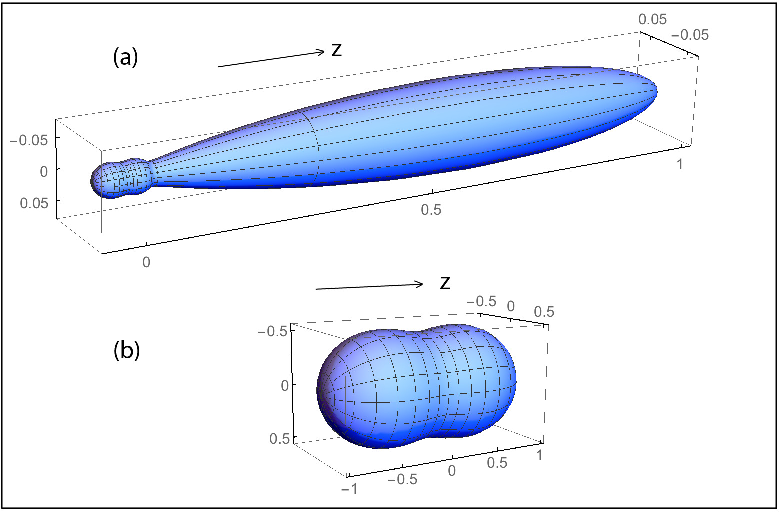
\includegraphics[width=\textwidth]{angular.pdf}
\end{center}
%\caption{Log-log plot of the total radiated power vs. the number of atoms from two types of models. $R$=1 and $\delta=600$ in both cases. The solid line is the result of Eq.~\eq{PN}. Ret dots denote the results from simulations.}
\caption{Normalized radiation patterns $P_N(\theta,R)\sin\theta$ for two Gaussian samples with $R=10$ in (a) and $R=0.1$ in (b). For both cases, the number of atoms is $N=20$, and the detuning is $\delta=600$.}
\label{ANGULAR}
\end{figure}

The main utility of these formulae is that they will serve as references with which to compare numerical results. A few incidental results could be noted, however.  The part $\propto N(N-1)$ in Eq.~\eq{PN} is the same as it would be for the continuous atom density in Eq.~\eq{CONT_DEN}, except for the factor of $N(N-1)$ instead of $N^2$. The intensity of the radiation in the forward direction, at $\theta=0$, coherent and incoherent components, add up to exactly $N^2$ times the intensity from a single atom. The bigger the sample, the narrower the cone in the direction $\theta=0$ for coherent scattering.  This aspect is demonstrated in Fig.~\ref{ANGULAR}. The sample acts as an antenna that directs the radiation in the forward direction. Nevertheless, the total power decreases with increasing size of the cloud.

Conversely, in the limit $R\rightarrow0$ the intensity in all directions is enhanced by a factor $N^2$, and of course so is the total power. Given the Dicke cooperative regime as discussed in Sec.~\ref{DICKESTORY}, a reader might erroneously interpret such an enhancement as a cooperative phenomenon. This cannot be, because in this example we have simply added the fields from independent radiators.

%Last but not least, the difference between the continuous medium model and the independent radiators model in the total scattering power is given by
%\bea
%P_N-P_C&=&\frac{N\left|\alpha\right|^2E_0^2}{3}\nonumber\\
%&&\cdot\left\{1-\frac{9\left[(4R^4-6R^2+9)-e^{-\frac{4R^2}{3}}(4R^4+6R^2+9)\right]}{32R^6}\right\}
%\label{diffNandC}
%\eea

\subsection{Simulation of the power in scattered light} 

When the dipolar fields from all the other radiators are taken into account, an analytical calculation for the total power is impractical and we have to utilize simulations. 

\begin{figure}[h!]
\begin{center}
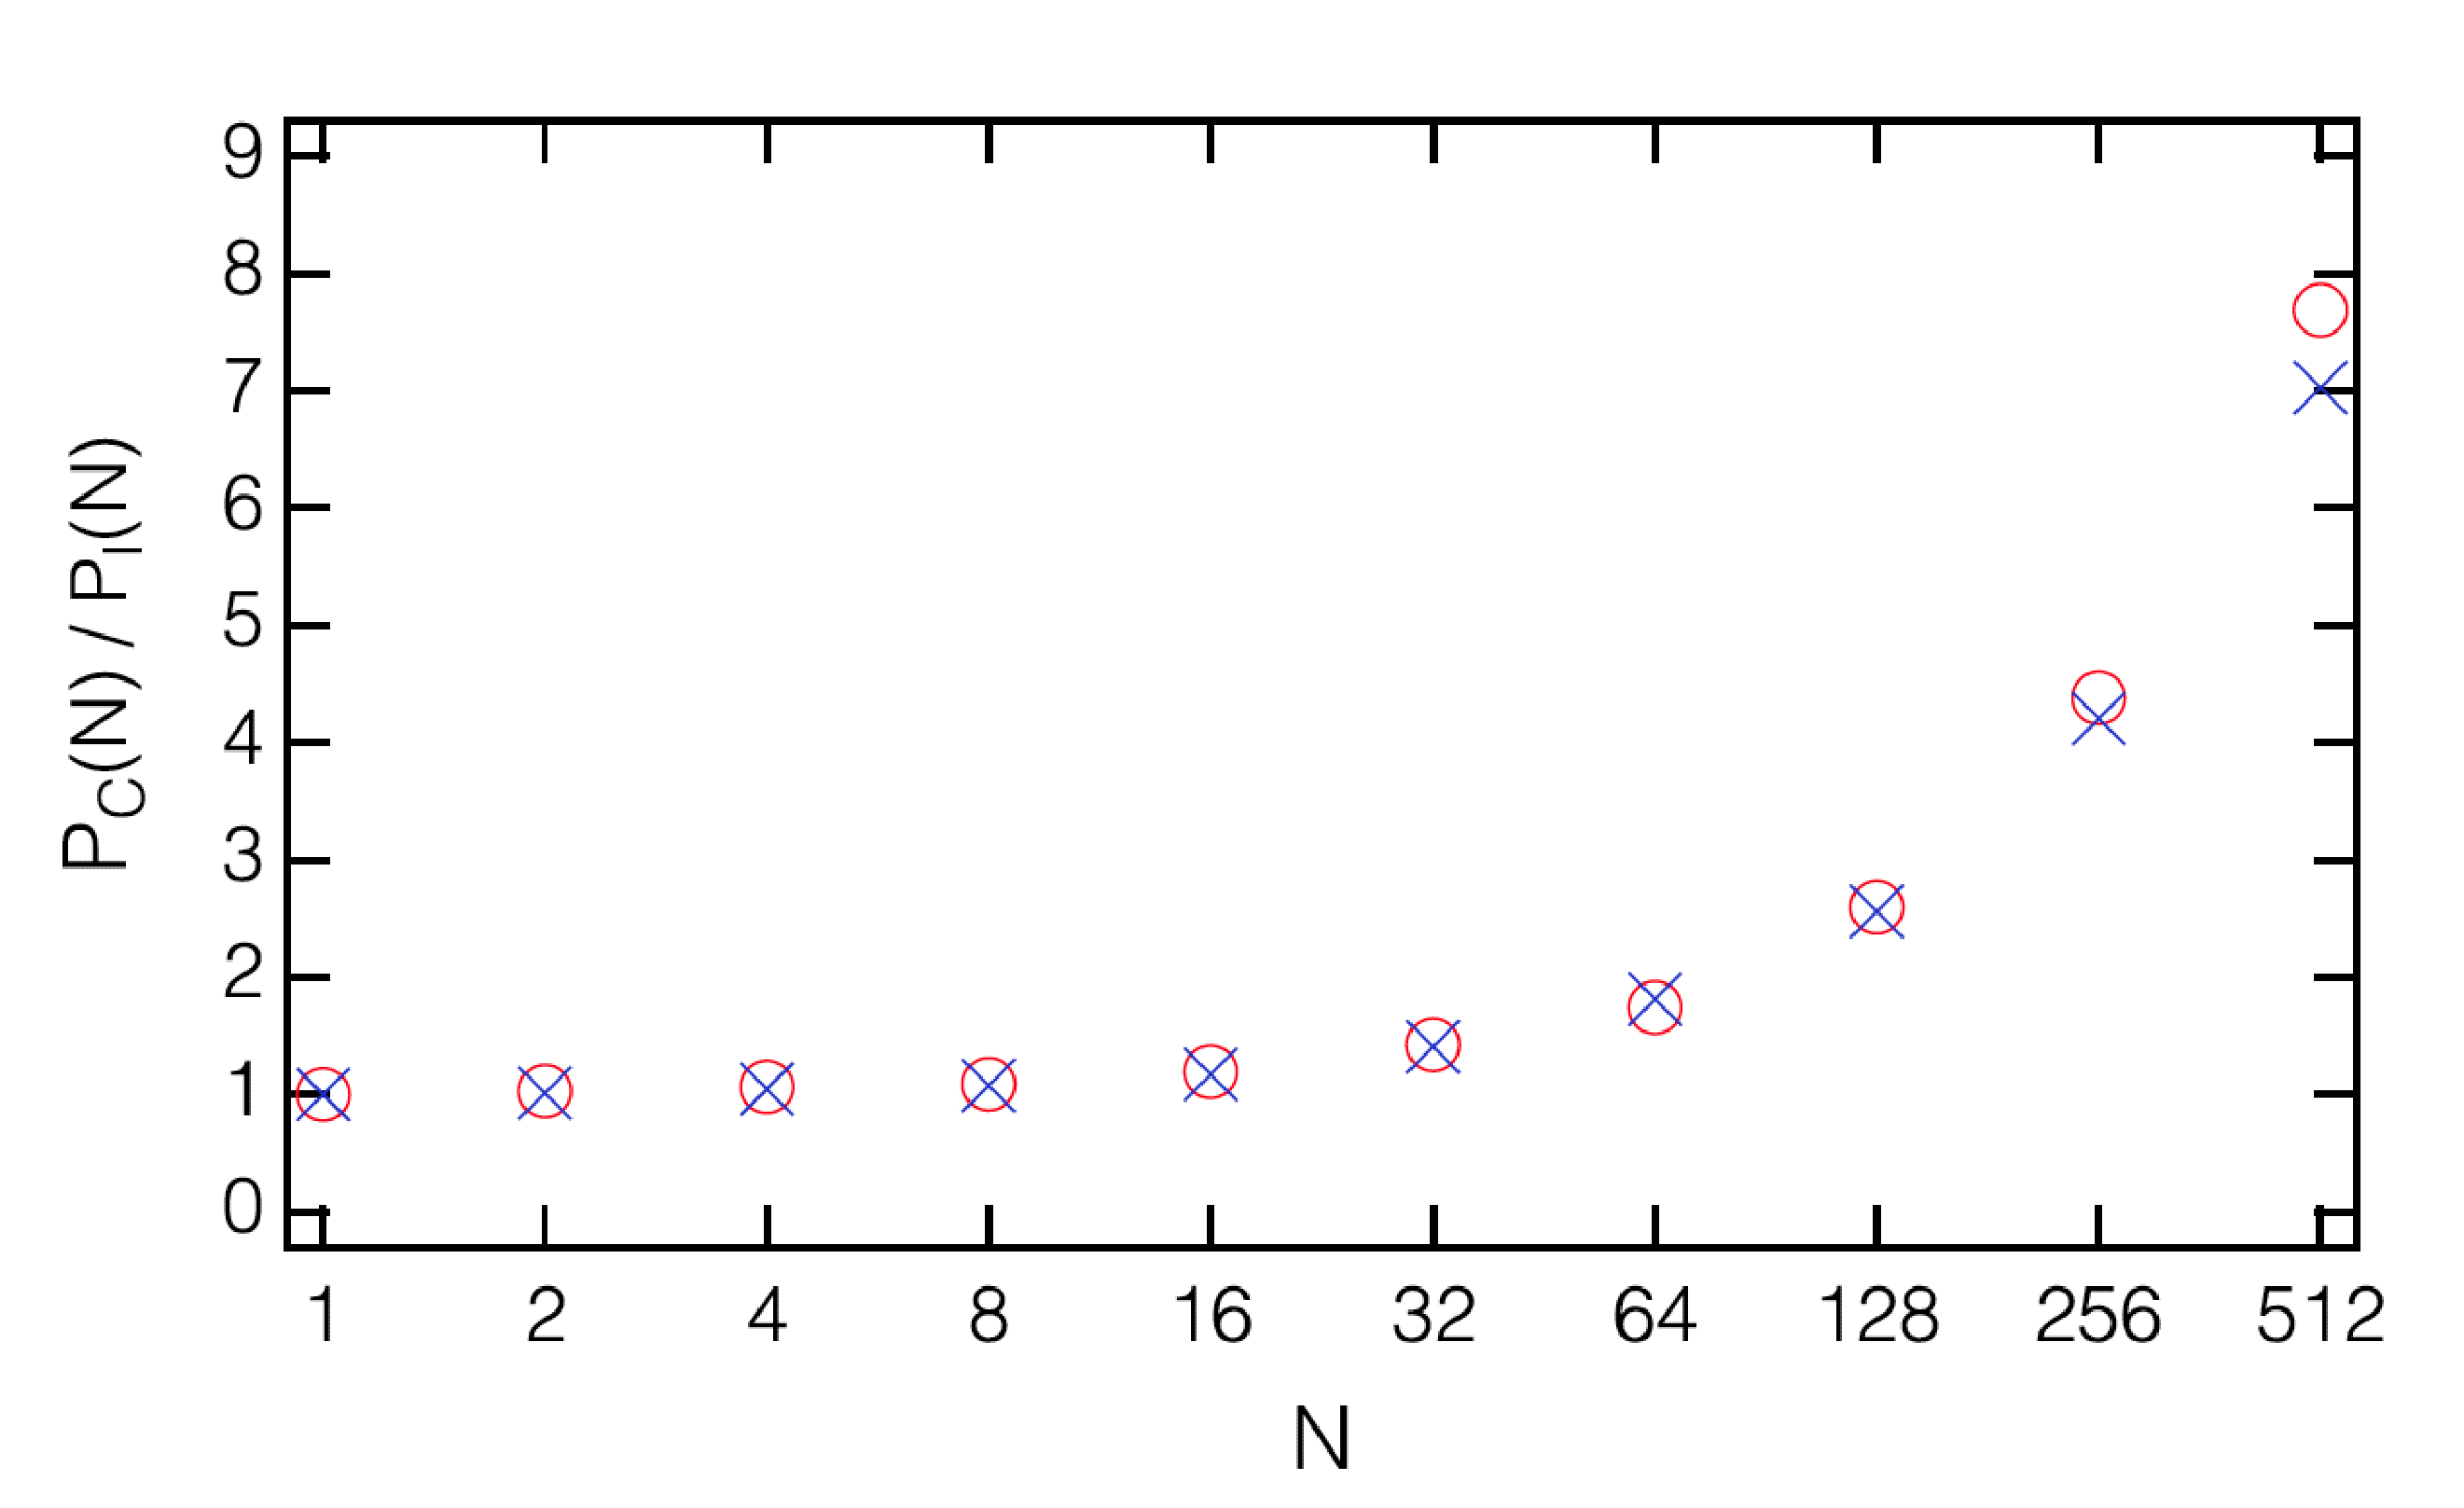
\includegraphics[width=\textwidth]{Pc_Pi.pdf}
\end{center}
%\caption{Log-log plot of the total radiated power vs. the number of atoms from two types of models. $R$=1 and $\delta=600$ in both cases. The solid line is the result of Eq.~\eq{PN}. Ret dots denote the results from simulations.}
\caption{Ratio of the numerically simulated scattered light power to the power from independently radiating atoms plotted for varying atom number $N$ for a Gaussian cloud with the rms radius $R$ satisfying $R=10$. The detuning is varied in such a way that the estimated optical thickness through the center of the cloud is $10^{-2}$ for all $N$. The circles and crosses are for different signs of the detuning, so that the cloud acts as either a focusing or a defocusing lens.}
\label{PCANDPN}
\end{figure}



We plot in Fig.~\ref{PCANDPN} the ratio of the numerically simulated collective power to the independent-atom power, $P_C(N)/P_I(N)$, for different numbers of the atoms $N$. Here the cloud radius is $R=10$. All of the data points are averaged over a large number of random positions of the atoms. While we vary the atom number and hence the density, we also vary the detuning in such a way that the estimated optical thickness for a ray of light going straight through the center of the cloud would be $10^{-2}$ so that absorption of light and indeed scattered dipole radiation should not be major factors. We have both positive (circles) and negative (crosses) detunings that make the gas either a focusing or defocusing lens.

The surprise here is that by $N=128$ when the collectively scattered power already more than doubles the independent-atom power, the central density is only $\rho=0.03$. We think that cooperative-operation sets in much earlier than expected, namely, around $\rho=1$, and we suspect that the same applies elsewhere too.


%The solid line in Fig.~\eq{PCANDPN} reflects the analytical result of a Gaussian cloud of independent radiators as given by Eq.~\eq{PN} and the red scatters represents the results of  radiators with dipole-dipole interactions.  
 
%We notice that the total power with cooperativity exceeds at small atom numbers but the situation reverses at large $N$, where the gas radiates much less then one would expect according to Eq.~\eq{PN}. This is a clear signature of cooperativity (for the only difference in this two models is the presence of light rescattering between atoms. ?)

\section{Shifts of resonance line in a circular disk}

Aside from total radiated power, spectroscopic evidence of cooperativity is also of interest to us. To study it, we replace the Gaussian cloud with a gas sample uniformly distributed inside a circular-disk shape container. This geometry has been addressed recently both in experiments and in theory~\cite{PhysRevLett.108.173601,Javanainen:16}.

The focus here is on the Lorentz-Lorenz (LL) shift and on the collective Lamb shift (CLS). 
We have summarized in Chapter 3 the argument from Ref.~\cite{FRIEDBERG1973101} that for a slab configuration, a uniform-density medium restricted to the interval $z\in [0,h]$, and for a plane wave with the wave number $k=\omega/c$ propagating in the $z$ direction, the absorption line should be shifted by
\bea
\Delta_L=\Delta_{LL}-\frac{3}{4}\Delta_{LL}\left(1-\frac{\sin 2hk}{2hk}\right);\,\quad\Delta_{LL}=-\frac{\rho\mathcal{D}^2}{3\epsilon_0\hbar} = -2\pi\rho k^{-3}\gamma
\label{LL_CLS}
\eea
from the atomic resonance. Here $\Delta_{LL}$, a redshift, is the standard LL shift, and $\Delta_L$ is the CLS as in Ref.~\cite{FRIEDBERG1973101}.  This is also the CLS verified in the experiments~\cite{PhysRevLett.108.173601}, albeit using hot atomic samples with moving atoms. As is obvious from Eq.~\eq{LL_CLS}, for the time being we have reverted to the standard SI units.

The original derivation of the CLS in Ref.~\cite{FRIEDBERG1973101}  was an elaborate QED argument. However, we now know~\cite{PhysRevLett.108.173601,Javanainen:16} that the same result can be obtained from the standard electrodynamics of polarizable media. The local-field corrections giving the $LL$ shift are inserted by hand as usual, while the oscillatory part $\propto\frac{3}{4}$ comes from etalon effects, reflections of light from the front and back surfaces of the slab. According to this argument, the LL shift should be there regardless, whereas the oscillatory part is valid in the limit of low atom density only.

In the face of the multitude of remarks pulling in different directions, it is of great interest to find out what the {\em exact\/} solution to the light propagation problem would say. That is why we solve the light propagation problem using stochastic classical-electrodynamics simulations~\cite{PhysRevA.59.649,PhysRevE.69.026605,PhysRevLett.101.103602,1367-2630-14-5-055001,PhysRevA.86.031602,PhysRevB.86.085116,PhysRevB.86.205128,PhysRevA.88.033844}. As discussed before, in the simulations we start with $N$ atoms fixed at positions $\br_i,\, i=1,\dots,N$, each with an assumedly isotropic polarizability $\alpha$, and form the closed set of linear equations~\eq{FEQ}. Having solved these equations numerically, at least in principle we have the electric field amplitude everywhere as in Eq.~\eq{EF}. This computation is done for a number of random positions of the atoms compatible with the geometry of the sample, and the results are averaged.

Of course a truly exact numerical solution for an infinite slab is impossible, as it would require infinitely many atoms. In the simulations reported in the present chapter we use a circular disk with the radius $R=\sqrt{256/\pi}k^{-1}$, so the area is $A=256k^{-2}$. We vary the thickness of the disk $h$ but keep the density $\rho=N/hA=2k^3$ constant in the examples of the present chapter, so that the number of atoms $N$ varies accordingly. A circularly polarized plane wave comes in perpendicular to the face of the disk. Analogous numerical experiments, although for different purposes, have been described in Refs.~\cite{1367-2630-14-5-055001,PhysRevA.86.031602}.  

A serious complication follows from the use of the finite-size disk, namely, diffraction. Extinction of light upon propagation through a sample means that the incoming and the reradiated light interfere destructively. A finite-size disk does not radiate a plane wave, so we lose what is known as mode matching between the radiation from the dipoles and the incoming plane wave. In fact, an exact computation of the transmitted light does not reproduce satisfactorily even the most rudimentary results of the optics of an infinite slab.

To circumvent this problem we resort to the method introduced in Ref.~\cite{1367-2630-14-5-055001}. Basically, we obtain the dipole moments of the atoms in the sample, but when calculating the field transmitted through the sample, we assume that each dipole radiates a plane wave that is automatically mode matched with the incoming wave. As before, let us assume that the incoming plane wave propagates in the $z$ direction. For a disk of radius $R$, the amplitude of the assumed plane wave from a dipole at ${\bf r}_j$ is computed as
\beq
\bE_j({\bf r}) = \frac{ik}{2\pi\epsilon_0 R^2} [\bd({\bf r}_j)-\hat{\bf e}_z \cdot\bd({\bf r}_j)\,\hat{\bf e}_z] e^{ik(z-z_j)}\,.
\label{TRLIGHT}
\eeq
This method produces good results even for a disk as small as the one we use in our simulations. In the limit of a dilute sample when we expect classical optics to apply, we get to within a few percent of the predictions of classical optics for an infinite slab.

We generate a number of random samples, from 64 to millions, of atomic positions evenly distributed inside the disk, compute the transmitted light as a function of the detuning $\Delta$ for each sample, and average the results. We report the optical thickness $D$ defined in terms of power transmission coefficient $T$ as $D=-\ln T$. The advantage here is that in a medium that obeys Beer's law the optical thickness would be linearly proportional to the thickness $h$, but would otherwise have the same line shape $D(\Delta)$ for all thicknesses. The scale of computations can be large; a publication-scale project can take $10^5$ hours of CPU time. The production runs we are discussing in the present chapter were mostly done on what is functionally a very large computer cluster, the Open Science Grid~\cite{OSG}.

Figure~\ref{HOMO_D} shows the optical thickness $D$ as a function of detuning $\Delta$ for the sample thicknesses $hk=0.25, 0.5, 1.0$ and $2.0$, with the corresponding atom numbers $N=128, 256, 512,$ and $1024$. For comparison we also give the predicted LL shift of this atom density as a dashed vertical line. The absorption lines are not Lorentzian. While the line broadens with increasing atom number and may be noticeably asymmetric, the maximum nevertheless moves very little. The shift, if any, is at most a few percent of the LL shift. No manifest LL shift is present, nor a CLS. Given that the LL shift comes from a universally accepted and widely used local-field arguments, its absence in the simulations is quite remarkable.


\begin{figure}[h!]
\begin{center}
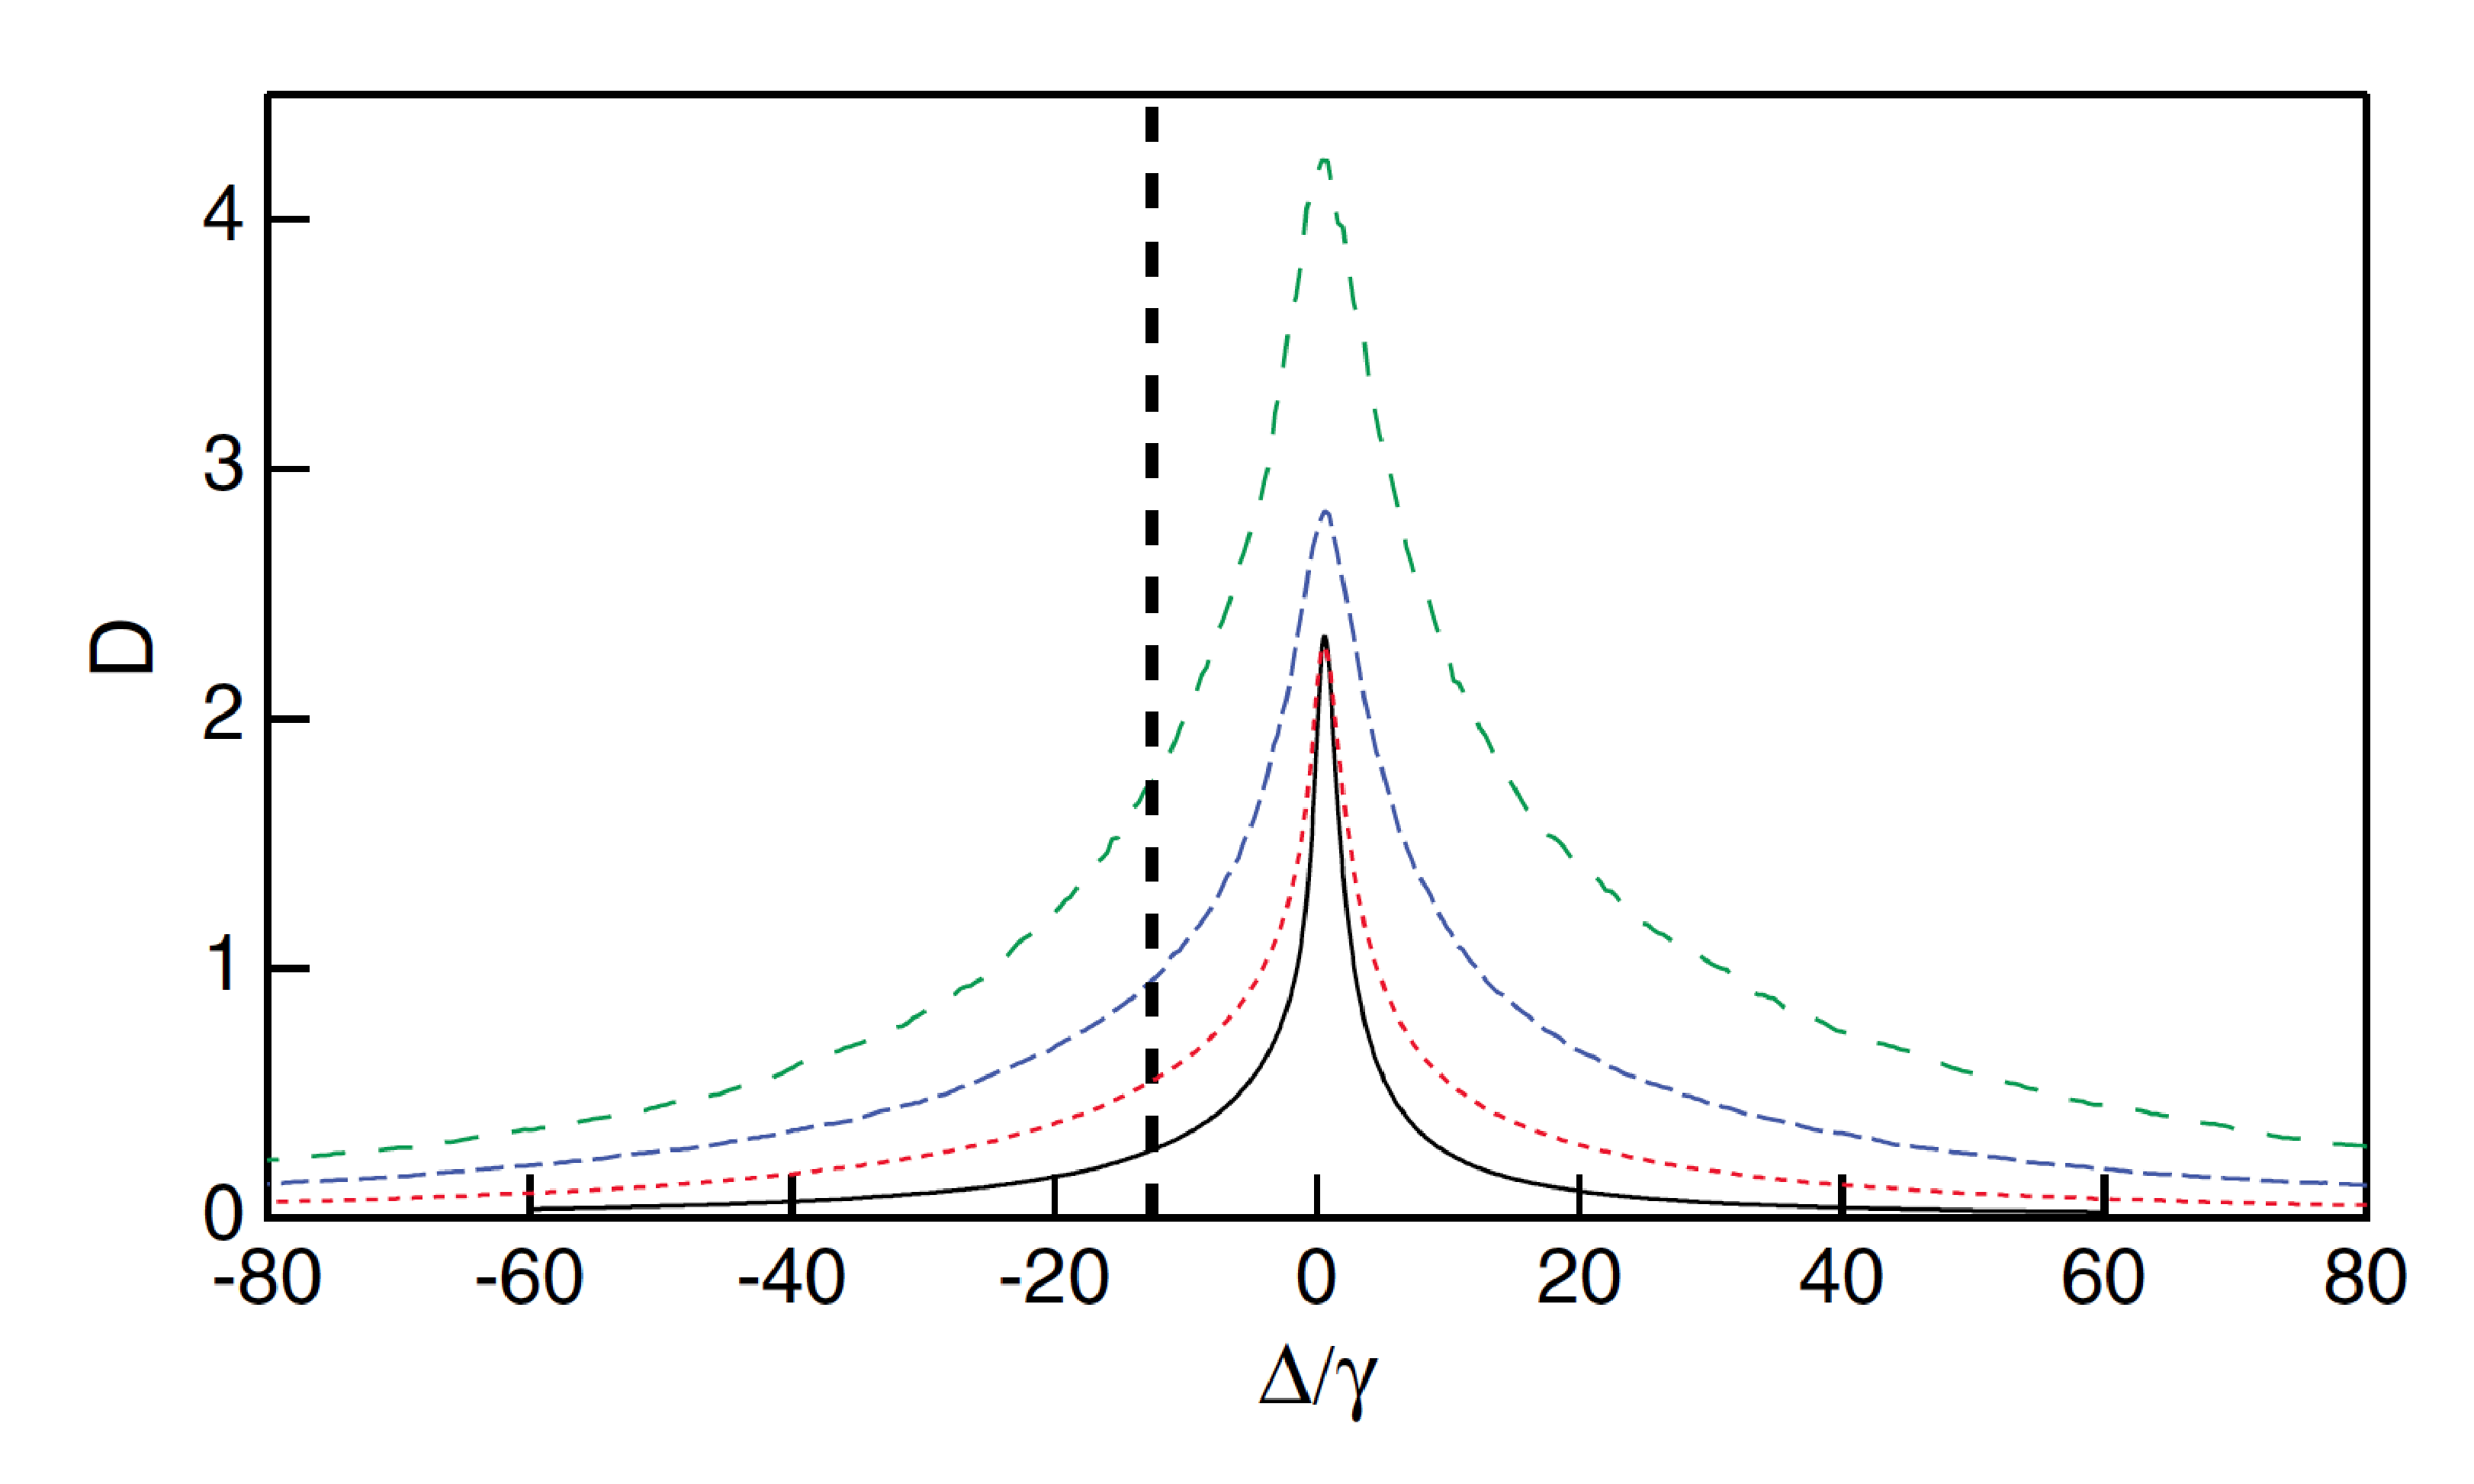
\includegraphics[width=\textwidth]{homo_D.pdf}
\end{center}
\caption{Optical depth $D$ versus detuning $\Delta$ for stationary atoms for sample thicknesses $hk=0.25, 0.5, 1.0$, and $2.0$, from bottom to top; the corresponding atom numbers are $N=128, 256, 512,$ and $1024$. The dashed vertical line shows where the center of the line would be if the naive Lorentz-Lorenz shift applied.}
\label{HOMO_D}
\end{figure}

Before introducing new factors into our simulations such as the actual motion of the atoms, we repeat the numerical experiments with stationary atoms in the circular disk. However, this time we assume that the resonance frequency of each atom is also shifted by a Gaussian random variable with zero mean and the rms value $\omega_D=100\gamma$. This is a basic model for the Doppler shifts that follow from the motion of the atoms. Given that we have a different resonance frequency for each atom, the atomic sample is termed ``inhomogeneously broadened''. In contrast, if the atoms are stationary or move so slowly that there is no significant effect on spectroscopy, as in our simulations until now, the sample is called ``homogeneously broadened''.

An example spectrum is shown in Fig.~\ref{INHOMO_D}. The line shape has an appearance common in the spectroscopy of inhomogeneously broadened samples. Accordingly, we fit it with the Voigt profile $V(\Delta-s;\Gamma,\Omega_D)$, convolution of a Lorentzian with the HWHM $\Gamma$ and a Gaussian with the rms width $\Omega_D$. We are particularly interested in the shift $s$ of the spectrum from the atomic resonance.

\begin{figure}[h!]
\begin{center}
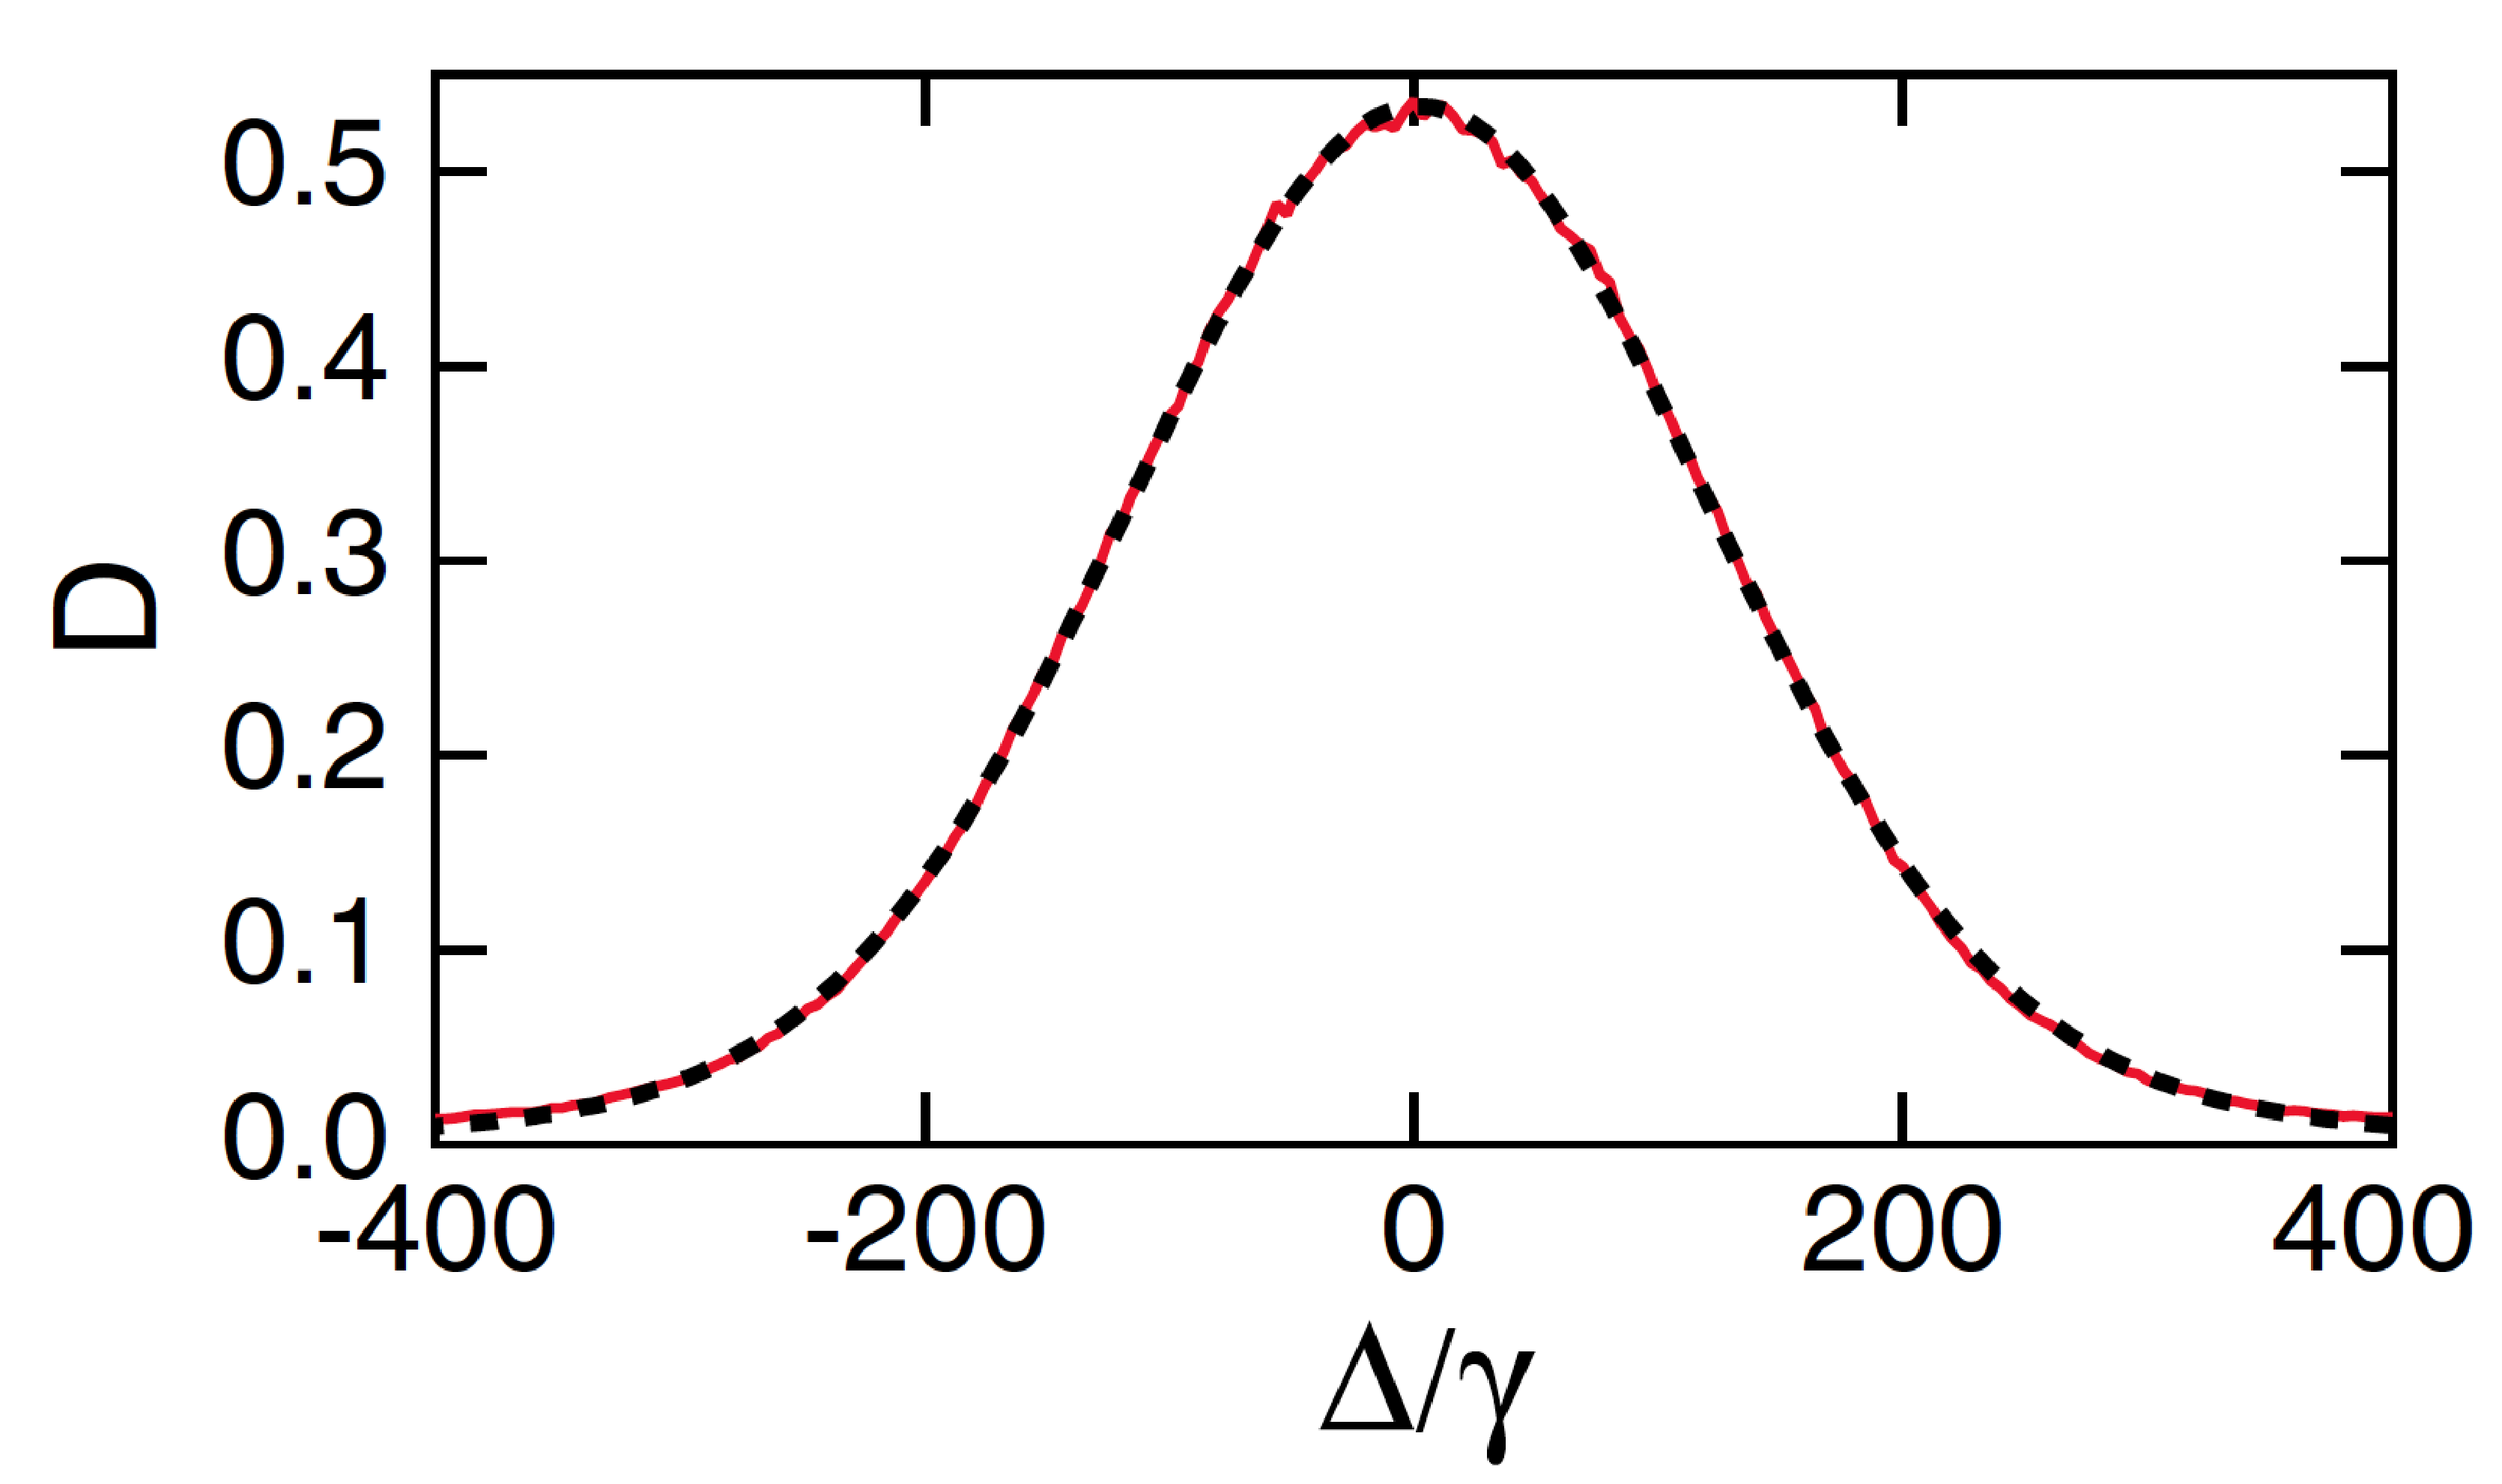
\includegraphics[width=\textwidth]{inhomo_D.pdf}
\end{center}
\caption{Optical depth of the sample $D$ with thickness $hk=1.5$, and, hence, $N=768$ atoms, as a function of the detuning for a sample with the inhomogeneous linewidth $\omega_D=100\gamma$. This numerical experiment (solid red line) is an average of 1024 samples, the fit with a Voigt profile (dashed black line) has the parameters $s=2.15\gamma$, $\Gamma=17.74\gamma$, and $\Omega_D=112.83\gamma$.}
\label{INHOMO_D}
\end{figure}

We plot the shift of the resonance $s$ for inhomogeneously broadened samples as a function of the thickness of the disk $h$ in Fig.~\ref{STATIC_CLS} as filled circles.  In these fits the widths of the Lorentzian and Gaussian components of the Voigt profile $\Gamma$ and $\Omega_D$ were also allowed to vary, and of course there was an overall multiplicative factor to fit.

The shift tends to zero at small thicknesses. In this limit the physics clearly becomes two dimensional, for a fixed three-dimensional density the relevant two-dimensional area density tends to zero, and eventually the atoms must radiate completely independently. 

We also plot the CLS, Eq.~\eq{LL_CLS}, as a solid line. Numerical data and theory show similar oscillations, albeit differing approximately by an additive constant. In Fig.~\eq{STATIC_CLS} we also plot as a dashed line the vertically translated version of the theory to fit the numerical data points with $hk\geq 1$. An additive term was also fitted to the experiments~\cite{PhysRevLett.108.173601} before they gave agreement with Eq.~\eq{LL_CLS}. The agreement of our numerical experiments with the CLS theory is on a similar footing as in the real experiments.


\begin{figure}[h!]
\begin{center}
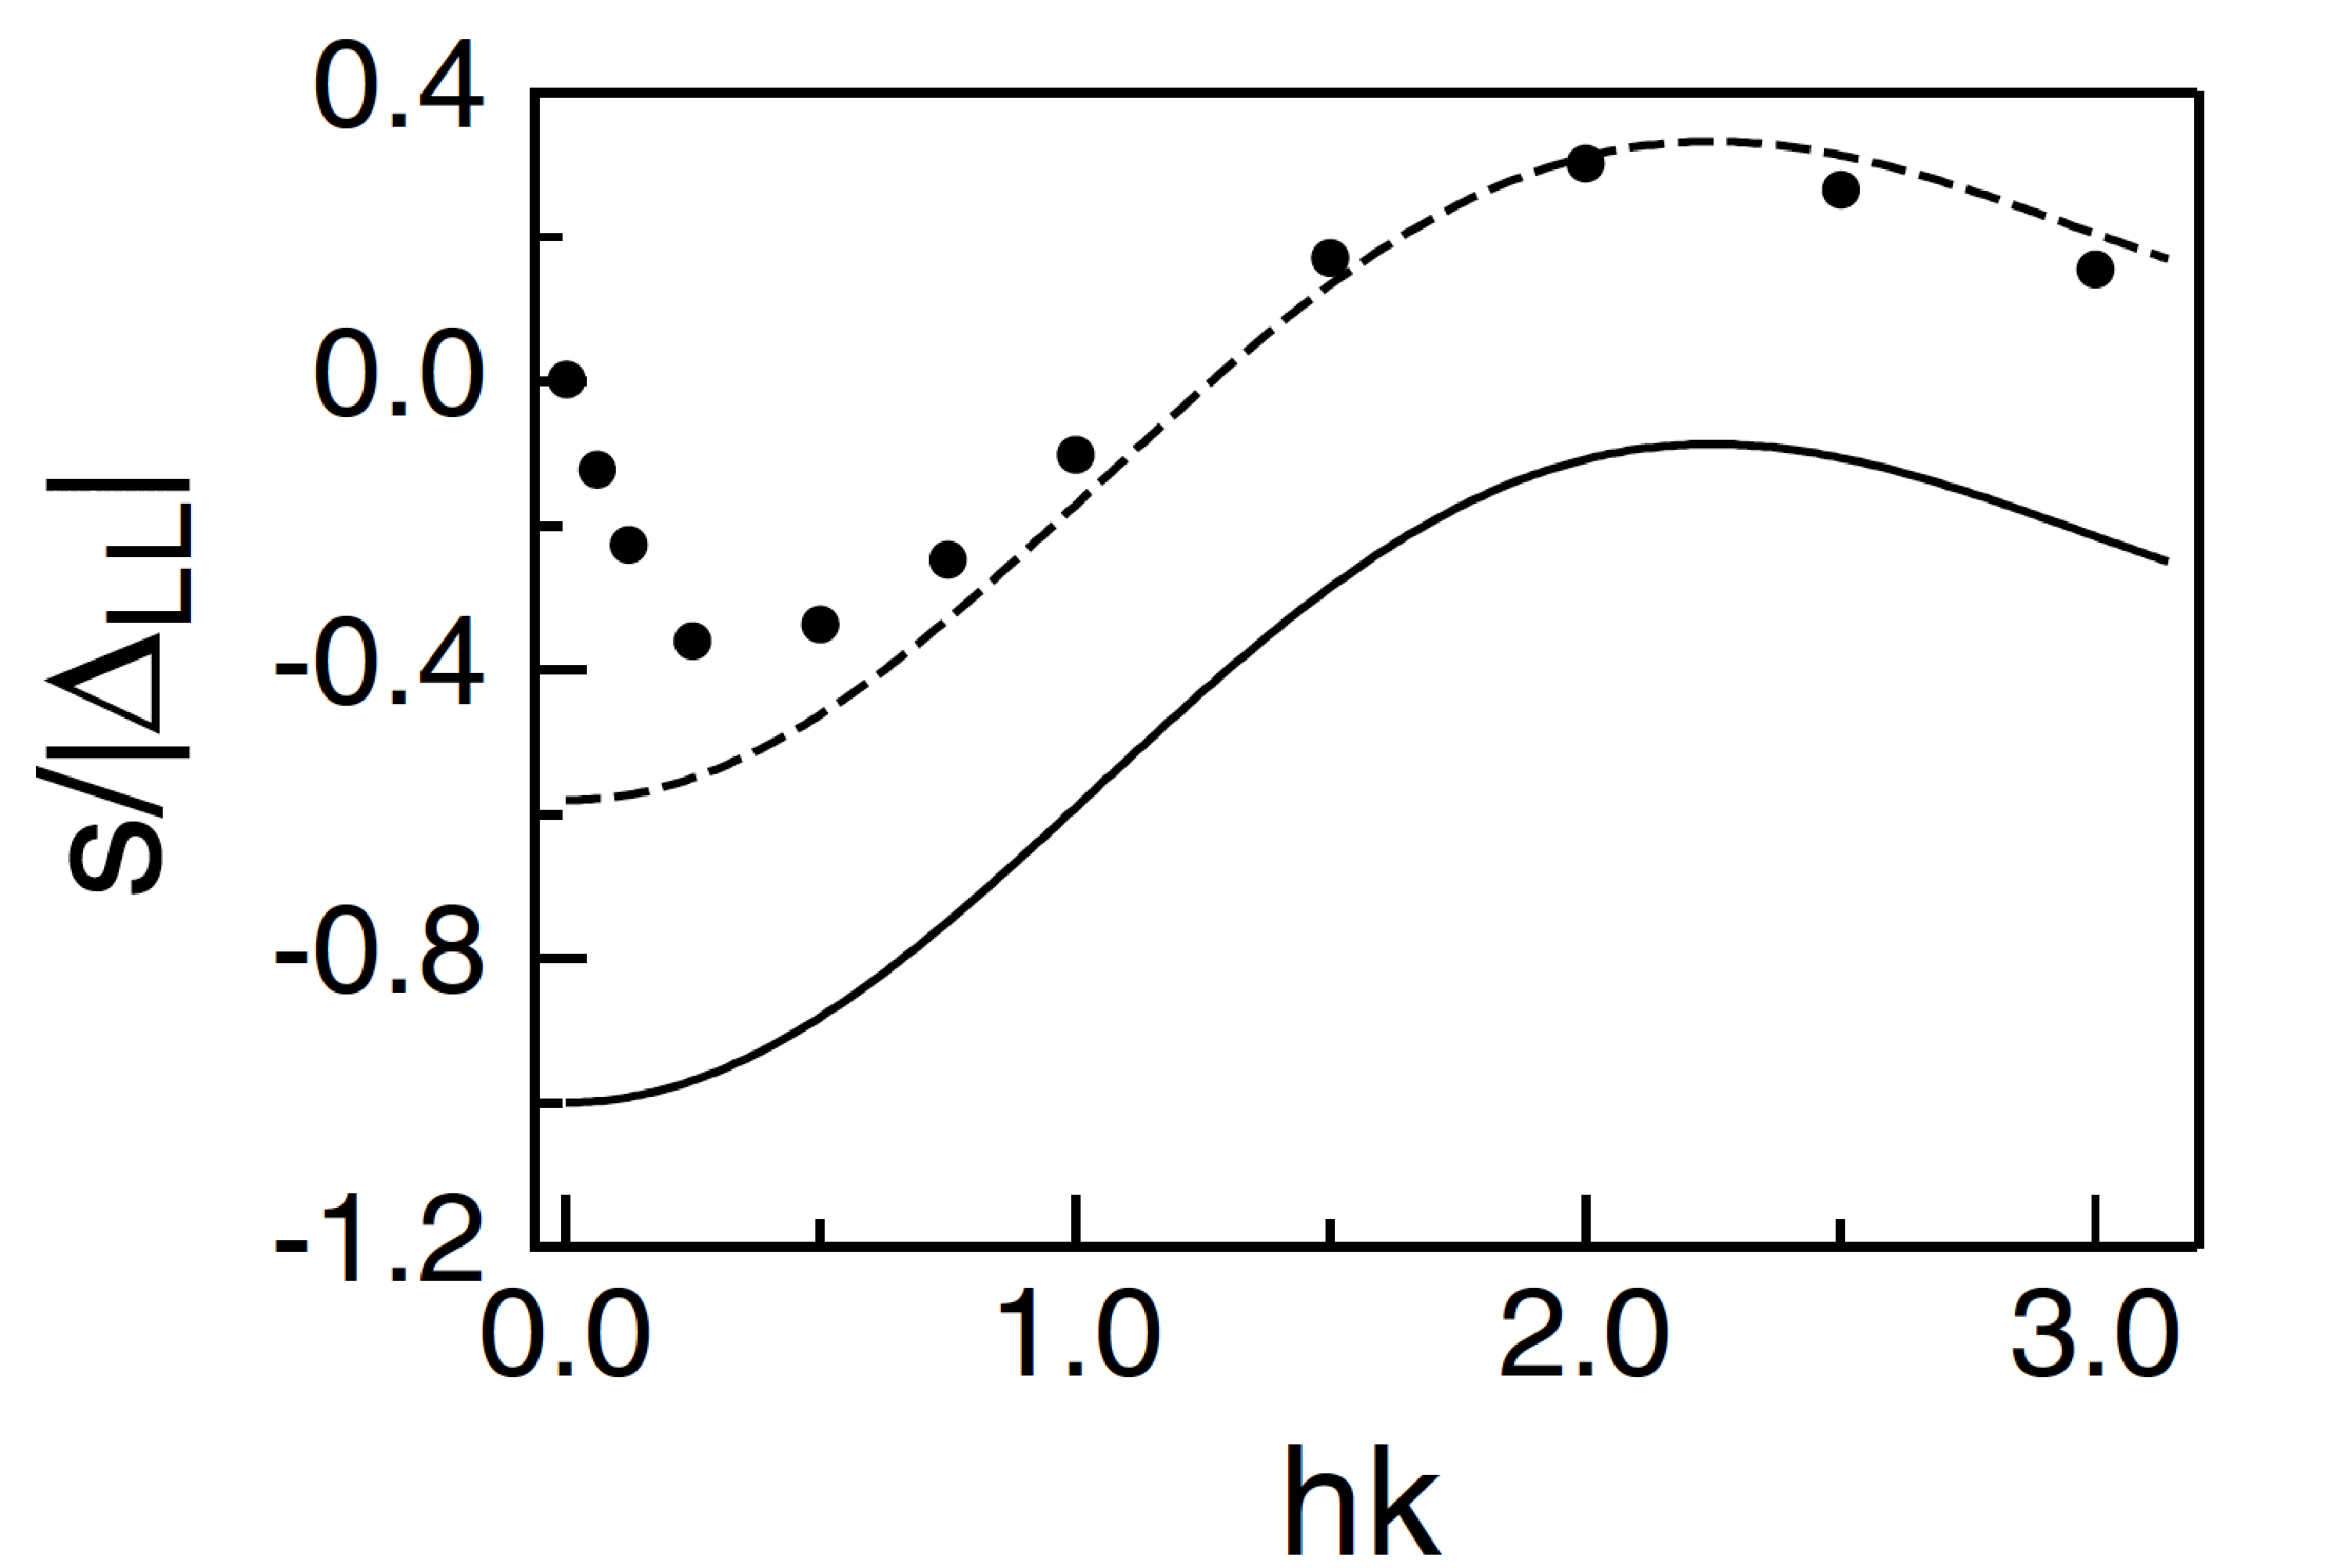
\includegraphics[width=\textwidth]{CLS_static.pdf}
\end{center}
\caption{The shift of the absorption line $s$ plotted as a function of the thickness of the sample $h$ as solid circles. The statistical error bars are smaller than the size of the circles. Also shown as a solid line is the collective Lamb shift, Eq.~\eq{LL_CLS}, and as a dashed line a vertically translated version of Eq.~\eq{LL_CLS} fitted to the numerical data points with $hk\geq 1$.}
\label{STATIC_CLS}
\end{figure}

Our interpretation is that for homogeneously broadened samples the standard electrodynamics, a mean field theory, simply fails. This is because at the density $\rho=2k^2$ the atoms are so close to one other that their dipole-dipole interactions make them a strongly interacting, or strongly correlated, system. On the other hand, inhomogeneous broadening appears to promote mean field physics.

For more insights, consider two atoms 1 and 2 with possibly different resonance frequencies, and hence, different polarizabilities $\alpha_1$ and $\alpha_2$. We sketch a formal solution to Eq.~\eq{FEQ}. The field on atom 2 that is generated by the incident field and the light scattered from atom 1 is
\bea
\bE(\br_2)&=&(1-\alpha_1\alpha_2\G\G)^{-1}[\cbE_0(\br_2)+\alpha_1\G\cbE(\br_1)]\nonumber\\
&=&\cbE_0(\br_2)+\alpha_1\G\cbE_0(\br_1)+\alpha_1\alpha_2\G\G\cbE_0(\br_2)+\dots.
\eea

The second line shows the first three terms of the expansion of $(1-\alpha_1\alpha_2\G\G)^{-1}$, with $\G\equiv\G(\br_1-\br_2)=\G(\br_2-\br_1)$. The first term is the free field on atom 2; in the second term the free field excites atom 1, which sends its dipolar field back on atom 2; in the third term the free field excites atom 2, which sends a dipolar field to excite atom 1, which sends a dipolar field back on atom 2. Further terms in the expansion come out in the same way reflecting repeated photon exchanges between the atoms. Such recurrent scattering processes in which a classical wave scatters more than once from the same atom is responsible for the cooperative phenomena and the emergence of subradiant and superradiant resonances~\cite{PhysRevA.55.513,PhysRevA.86.031602,PhysRevB.86.085116}.

Let us now regard atom 2 as the spectator and imagine averaging over the position of atom 1. Upon averaging, the second term becomes the mean-field contribution radiated by an assumedly continuous polarization, and further terms represent repeated photon exchanges between the atoms. 

Next, add the inhomogeneous broadening $\omega_D$. To the order of magnitude, averaging over the resonant frequencies suppresses the polarizability by a factor of $\gamma/\omega_D$. Thus, the first nontrivial term in the expansion corresponding to the mean-field polarization becomes suppressed by this factor, and the higher terms by higher powers of the small quantity $\gamma/\omega_D$. Qualitatively, repeated photon exchanges are deemphasized because in such processes both the emitter and the absorber are off resonance. This leaves the mean field as the dominant contribution.

Analogously, the transition from homogeneously broadened to inhomogeneously broadened phenomenology also takes place in a many-atom sample when the inhomogeneous broadening $\omega_D$ and the effective linewidth $\Gamma$ are comparable. This is, in fact, what we observe in the numerical experiments.

From classical-electrodynamics simulations, we have found qualitative features in the optical response of a homogeneously broadened dense atomic sample that are at variance with the time-honored pictures of local-field corrections and collective Lamb shifts. However, an inhomogeneous broadening, random distribution of atomic resonance frequencies, restores the agreement with the traditional theory at least in part.

So far, the simulations are based on atoms fixed in their positions, with at best a crude model for inhomogeneous broadening. In the following chapter, the actual motion of the atoms will be introduced into the simulations.

